%\documentclass[a4paper,11pt,fleqn]{report}
%\documentclass[a4paper,11pt,twoside]{report}
\documentclass[a4paper,12pt,]{report}
\usepackage[utf8x]{inputenc}
\usepackage[T1]{fontenc}
\usepackage[german, ngerman]{babel}
\usepackage{longtable}
\usepackage[BCOR0.5cm]{typearea} %deaktivate
\usepackage{tabularx}
\usepackage{latexsym}
\usepackage{amsmath,mathptmx} %  Times-Schriftart
\usepackage{graphicx,float}
\usepackage{helvet}
\usepackage{fancyheadings}
\pagestyle{fancy}
\usepackage{geometry}
\usepackage{microtype}
\geometry{a4paper, top=30mm, left=25mm, right=25mm, bottom=0mm,
headsep=10mm, footskip=10mm}
%\usepackage{amsfonts}
\usepackage{listings}
\setlength{\headwidth}{16cm}
\setlength{\textwidth}{16cm}
\setlength{\leftmargin}{-1cm}

\renewcommand{\chaptermark}[1]%
                  {\markboth{#1}{}}

\renewcommand{\sectionmark}[1]%
               {\markright{\thesection\ #1}}
\lhead[\fancyplain{}{\bfseries\thepage}]%
     {\fancyplain{}{\bfseries\rightmark}}
\rhead[\fancyplain{}{\bfseries\leftmark}]%
      {\fancyplain{}{\bfseries\thepage}}
\cfoot{}

\setlength{\parindent}{0pt} %kein einzug nach Absatz

\renewcommand{\baselinestretch}{1.2} 
\usepackage{lscape} 
\setlength{\textheight}{24.5cm}

%\usepackage[hang, rm, bf]{caption}
\usepackage[font=small,format=plain,labelfont=bf,up,textfont=rm,rm]{caption}
\clubpenalty = 10000 
\widowpenalty = 10000 
\displaywidowpenalty = 10000
\usepackage{hyperref}
\begin{document}

\thispagestyle{empty}


\begin{figure}[t]
\vspace{-3cm}
\begin{minipage}[t]{3cm}
\vspace{-2cm}

\includegraphics[width=6cm]{Deckblatt/Wortmarke_RUB.jpg}
\end{minipage}
\hfill
\begin{minipage}[t]{3cm}

\includegraphics[width=3cm]{Deckblatt/Label_RUB.jpg}
\end{minipage}
\vspace{3cm}
\end{figure}


\renewcommand{\rmdefault}{phv}
\begin{center}


	{\Huge \bf P R O J E K T A R B E I T}
	
	\vspace{0.5cm}
	
	{\Large
	zum Thema:\\
	\vspace{0.5cm}
	Entwicklung eines Server-Client Systems zur Darstellung PDF-basierter Präsentationen\\
	\vspace{0.5cm}
	von\\
	\vspace{0.5cm}
	{\LARGE \bf
	René Beckmann\\
	Sascha Brexeler\\
	Diana Castano\\
	Tim Hebbeler\\
	Jens Helge Micke\\
	}
	\vspace{0.5cm}
	}
\end{center}

\begin{table}[h!]
\begin{tabular}{p{0.5\textwidth}p{0.5\textwidth}}
Betreuender Dozent & Dr. Wolfgang Theimer\\
&\\
&\\
&\\
&\\
&\\
Beginn: & 13.04.2016\\
&\\
Abgabe: & 20.07.2016\\
\end{tabular}
\end{table}

\renewcommand{\rmdefault}{ptm}

\pagenumbering{Roman}
\setcounter{secnumdepth}{3}
\setcounter{tocdepth}{2}
{\parskip=4mm \tableofcontents}
\newpage
\listoffigures
\newpage
\pagenumbering{arabic}

%\include{Erklaerung/Erklaerung}

\setcounter{page}{1}

\chapter{Einleitung}
\thispagestyle{fancy}


\chapter{Projekt und Organisation}
\thispagestyle{fancy}
\label{ProjektOrganisation}
Inhalt dieses Kapitels ist die Vorstellung des Projektes und die Organisation der Gruppe 4.
\section{Das Projekt}
\label{DasProjekt}
Die Entwicklung eines Server-Client Systems zur Darstellung PDF-basierter Präsentationen kristallisierte sich nach der Abwägung anderer Projektmöglichkeiten\footnote{Besprochene Alternativen: Ein kooperatives Jump 'n Run Spiel, Medienserver} heraus.
Auch, dass der ausgehändigte \glqq Raspberry Pi 3 \grqq als Server und, in Verbindung mit einer HDMI-fähigen Anzeige, als Primäranzeige dienen soll ergab sich als natürliche Rahmenbedingung.
\subsection{Anwendungsfälle}
\label{Anwendungsfälle}
Bevor es an die Verteilung von Aufgaben innerhalb des Projektes ging wurden die entsprechenden Anwendungsfälle erarbeitet.
Während der Realisierung wurden diese an die derzeitige Situation angepasst und nötigenfalls Erweitert.\\


\begin{tabular}{|r|l|}
	\hline
	1.0 & Präsenter \\
	 & Mehrere Personen wollen eine Präsentation halten \\
	\hline
	\hline
	1.1 & PräsenterEinwahl\\
	& Präsenter wählt sich in das System ein\\
	\hline
	\hline
	1.2 & PräsentationHochladen\\
	& Präsenter lädt Präsentation hoch\\
	VORRAUSSETZUNG & 1.1 PräsenterEinwahl\\
	\hline
	\hline
	1.3 & PräsentationAnzeigen\\
	& Die Präsentation wird angezeigt\\
	VORRAUSSETZUNG & 1.2 PräsentationHochladen\\
	\hline
	\hline
	1.4 & Navigation\\
	& Präsenter navigiert Präsentation\\
	BEFEHLE & vor, zurück\\
	VORRAUSSETZUNG & 1.3 PräsentationAnzeigen\\
	BESCHRÄNKUNG & Anfang/Ende der Präsentation\\
	BESCHRÄNKT & 2.2 PräsentationAnzeigen\\
	\hline
	\hline
	1.4.1 & NavigationSchaltflächen\\
	& Benutzeroberfläche stellt NavigationSchaltflächen bereit\\
	BEFEHLE & wie 1.3\\
	\hline
	\hline
	1.4.2 & NavigationBeschleunigungssensor\\
	& Navigation durch Kippbewegungen\\
	BEFEHLE & zurück, vor\\
	BESCHRÄNKUNG & Orientierung des Geräts\\
	\hline
	\hline
	1.4.3 & NavigationMikrofon\\
	& Navigation durch Klopfzeichen\\
	BEFEHLE & 1x Klopfen = vor\\
	& 2x Klopfen = zurück\\
	\hline
	\hline
	1.4.5 & NavigationKamera\\
	& Kamera erkennt Gesten zur Navigation\\
	BEFEHLE & Bewegung nach links = zurück\\
	& Bewegung nach rechts = vor\\
	\hline
	\hline
	1.5 & Menue\\
	& Navigationsmöglichkeiten 1.4.x x>1 an/abschalten\\
	& Die Präsentation kann beendet werden.\\
	& Eine neue Präsentation kann gestartet werden.\\
	\hline
\end{tabular}

\begin{tabular}{|l|l|}
	\hline
	2.0 & Publikum\\
	& Mehrere Personen wollen eine Präsentation verfolgen\\
	\hline
	\hline
	2.1 & PublikumEinwahl\\
	& Publikumsperson wählt sich in das System ein\\
	\hline
	\hline
	2.2 & PräsentationAnzeigen\\
	& Die Präsentation wird angezeigt\\
	VORRAUSSETZUNG & 1.3 PräsentationHochladen\\
	& 2.1 PublikumEinwahl\\
	\hline
	\hline
	2.3 & PräsentationSpeichern\\
	& Die Präsentation wird gespeichert\\
	VORRAUSSETZUNG & 1.3 PräsentationHochladen\\
	& 2.1 PublikumEinwahl\\
	\hline
	\hline
	2.4 & Verlassen\\
	& Die Publikumsperson verlässt die Präsentation\\
	VORRAUSSETZUNG & 2.1 PublikumEinwahl\\
	\hline
	\hline
	2.5 & Menue\\
	& Ein Menue erlaubt die Anwendungsfälle 2.1 - 2.4\\
	\hline
\end{tabular}

\begin{tabular}{|l|l|}
	\hline
	3.0 & DienstAnforderungen\\
	\hline
	\hline
	3.1 & Benutzer/Rechteverwaltung\\
	& Mehrere Präsenter\\
	& Mehrere passwörgeschützte Publikumspersonen\\
	\hline
	\hline
	3.2 & Datenverwaltung\\
	& Sortierung und Verwaltung von Präsentationen\\
	\hline
	\hline
	3.3 & Klientenschnittstelle\\
	& Muss derzeitige Seite der Präsentation verteilen.\\
	\hline
	\hline
	3.4 & Klientenverteilung\\
	& Muss aktuellste Version des Klienten verteilen\\
	\hline
\end{tabular}

\begin{figure}[ht!]
	\centering
	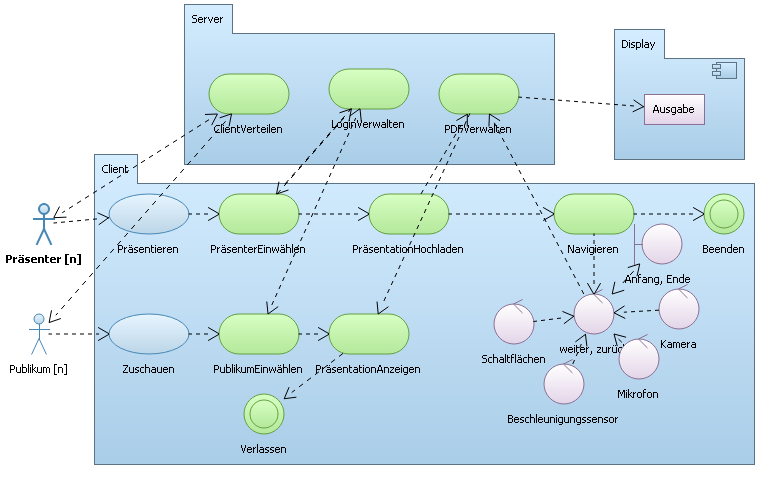
\includegraphics[angle=0,width=14cm]{ProjektOrganisation/Bilder/Anwendungsfaelle.png}
	\caption{Anwendungsfälle}
	\label{BildAnwendungsfaelle}
\end{figure}

\section{Die Organisation}
Aus den Anwendungsfällen in Kapitel \ref{Anwendungsfälle} Seite \pageref{Anwendungsfälle} ff. bzw. Bild \ref{BildAnwendungsfaelle} Seite \pageref{BildAnwendungsfaelle} ließen sich erste Hauptverantwortlichkeiten der Gruppenmitglieder ableiten und verteilen.\\

\begin{tabular}{|l|l|}
	\hline
	Server & Entwicklung des Servers\\
	\hline
	Klient & Benutzeroberfläche und Serverandbindung \\
	\hline
	Navigation & Navigationsmöglichkeiten\\
	& Berührungsschaltflächen, Kamera, Beschleunigungssensor, Mikrofon\\
	\hline
	Raspberry Pi & Integration auf der Hardware\\
	& Klientenverteilung\\
	\hline
	Dokumentation & Projektdokumentation\\
	\hline
	PDF-Renderer & Bereitstellen des PDF-Renderers\\
	\hline
\end{tabular}
\\
\begin{tabular}{|l|l|}
	\hline
	René Beckmann & Server\\
	& Klient Serveranbindung\\
	\hline
	Sascha Brexeler & Klient Benutzeroberfläche\\
	& Navigation Berührungsschaltflächen\\
	\hline
	Diana Castano & Navigation Mikrofon\\
	\hline
	Tim Hebbeler & PDF-Renderer\\
	& Navigation Kamera\\
	\hline
	Jens Helge Micke & Raspberry Pi\\
	& Navigation Beschleunigungssensor\\
	& Dokumentation\\
	\hline
\end{tabular}
\\
GitHub.com\footnote{https://github.com/BeckmaR/EmbeddedMultimediaSS2016} wurde als Versionsverwaltungsplatform genutzt.\\
Absprachen geschahen über regelmäßige Treffen und Gruppenchat.\\
Die zu bearbeitenden Projektteile wurden in kleinen Modulen entwickelt, getestet und nacheinander zusammengefügt.\\
Zu diesem Zweck traf sich die Gruppe zusätzlich zur Heimarbeit zu mehreren Test- und Programmierwochenenden bei denen die Gruppenmitglieder sich gegenseitig halfen und die bearbeiteten Problemlösungen testeten.\\
\chapter[Hardware]{Hardware\footnote{Jens Helge Micke}}
\thispagestyle{fancy}
\label{Hardware}
Dieses Kapitel behandelt die Eingesetzte Hardware und deren Konfiguration.
\section{Raspberry Pi 3}
\label{HardwareRaspberryPi3}
Zur Bearbeitung des Projektes wurde an jede Gruppe ein\glqq Raspberry Pi 3\grqq inklusive einer 16GB MicroSD Karte verteilt.\\
In diesem Projekt wurde der \glqq Raspberry Pi 3\grqq als Server, Verteiler, Zugangspunkt und Primäres Display genutzt.\\
Dazu mussten Debian, QT5.7, QTCreator 4.0.2, hostapd, dnsmasq, lighttpd, die in Kapitel installiert und, wie in den weiteren Abschnitten erläutert, eingestellt werden.
\subsection{Debian}
Als Betriebssystem kam die neueste für den Raspberry Pi angepasste Debian Version namens \glqq Raspbian\grqq zum Einsatz.\\
Diese wird als Abbilddatei zur Verfügung gestellt und lässt sich Problemlos auf die Ausgeteilte SD Karte brennen.\\
\subsubsection{Hindernisse}
Zum Reibungslosen Betrieb des Debian Systems sind einige Hindernisse zu überwinden.
\paragraph{Stromsparmodus}$\;$\\
Ein bekanntes Problem der Raspbian Distribution ist, dass ein verdunkeln und Abschalten des Bildschirms nicht immer mit den gängigen Methoden zu unterbinden ist.\\
Abhilfe schafft das Ausnutzen eines anderen bekannten Fehlers. Dazu muss das Programm xscreenserver installiert und in seinen Einstellungen deaktiviert werden. Dadurch beendet sich xscreenserver bei seinem Aufruf selbst und der Bildschirm kann nicht verdunkeln.
\paragraph{HDMI Kompatibilität}$\;$\\
Bei Tests mit unterschiedlichen Bildschirmen ist aufgefallen, dass der experimentelle openGL Treiber nicht mit älteren Geräten kompatibel ist.\\
Um diesen Abzuschalten ist darauf zu achten, dass in der /boot/config.txt die Zeile dtoverlay=vc4-kms-v3d ausgeblendet ist.\\
Um weiter die Verträglichkeit mit älteren Bildschirmen zu erhöhen lässt sich die Auflösung des HDMI-Ausganges auf VGA begrenzen. Dies ermöglicht auch, dass das Gerät ohne Bildschirm betrieben werden kann.\\
Dazu muss in der bereits Erwähnten /boot/config.txt der Eintrag hdmi\textunderscore force\textunderscore hotplug=1 aktiviert sein.\\
Für weitere Einstellungsmöglichkeiten sei an dieser Stelle auf die Kommentare in der /boot/config.txt und die Raspbian Dokumentation verwiesen.
\subsection{QT5.7}
Für dieses Projekt wurde die zu dieser Zeit neu herausgekommene QT Version 5.7 benutzt. Da jedoch nur QT 5.3 in den Debian Jessie Bezugsquellen integriert wurde musste diese händisch kompiliert werden.
\paragraph{Vorbereitungen}$\;$\\
Da die Dokumentation des Herstellers zur händischen Kompilierung nicht vollständig ist wird diese hier ohne die Integration des WebKit skizziert.\\
Dieser Vorgang benötigt zwischen 10 und 20 Stunden.

\begin{lstlisting}[frame=single,breaklines=true,basicstyle=\tiny,language=C,label={QT5.7compile},caption={Skizze zur Installation von Qt5.7}]
Das Dateisystem auf die gesamte 16GB SD Karte erweitern.
sudo raspi-config
---
Auslagerungsdatei auf 2GB erweitern 
sudo nano /etc/dphys-swapfile 
CONF\textunderscore SWAPSIZE=2048 

sudo dphys-swapfile setup 
---
Sicherstellen, dass die Folgenden Dateien gefunden werden:
sudo ln -s /opt/vc/include/interface/vcos/pthreads/vcos_futex_mutex.h /opt/vc/include/interface/vcos/vcos_futex_mutex.h
sudo ln -s /opt/vc/include/interface/vcos/pthreads/vcos_platform.h /opt/vc/include/interface/vcos/vcos_platform.h
sudo ln -s /opt/vc/include/interface/vcos/pthreads/vcos_platform_types.h /opt/vc/include/interface/vcos/vcos_platform_types.h
sudo ln -s /opt/vc/include/interface/vmcs_host/linux/vchost_config.h /opt/vc/include/interface/vmcs_host/vchost_config.h
---
Sicherstellen, dass die richtigen openGLES Treiber geladen werden:
sudo mv /usr/lib/arm-linux-gnueabihf/libEGL.so.1.0.0  /usr/lib/arm-linux-gnueabihf/libEGL.so.1.0.0.backup
sudo mv /usr/lib/arm-linux-gnueabihf/libGLESv2.so.2.0.0 /usr/lib/arm-linux-gnueabihf/libGLESv2.so.2.0.0.backup
sudo ln -s /opt/vc/lib/libEGL.so /usr/lib/arm-linux-gnueabihf/libEGL.so.1.0.0
sudo ln -s /opt/vc/lib/libGLESv2.so /usr/lib/arm-linux-gnueabihf/libGLESv2.so.2.0.0
---
Laden und entpacken von QT5.7.0
mkdir /home/pi/opt
cd /home/pi/opt
wget http://download.qt.io/official_releases/qt/5.7/5.7.0/single/qt-everywhere-opensource-src-5.7.0.tar.gz
mkdir -p /home/pi/opt/qt-everywhere-opensource-src-5.7.0
ln -s /home/pi/opt/qt-everywhere-opensource-src-5.7.0 /home/pi/opt/qt5
tar zxvf /home/pi/opt/qt-everywhere-opensource-src-5.7.0.tar.gz
---
Pfade anpassen
nano /home/pi/setup_qt.sh
export LD_LIBRARY_PATH=/usr/local/qt5/lib
export PATH=/usr/local/qt5/bin:$PATH

nano /home/pi/setup_general.sh
export PKG_CONFIG_PATH=/usr/lib/arm-linux-gnueabihf/pkgconfig
---
und automatisch laden
echo source /home/pi/setup_qt.sh >> /home/pi/.bashrc
echo source /home/pi/setup_qt.sh >> /home/pi/.profile
echo source /home/pi/setup_general.sh >> /home/pi/.bashrc
echo source /home/pi/setup_general.sh >> /home/pi/.profile
---
Abhaengigkeiten installieren:
sudo apt-get install libfontconfig1-dev libdbus-1-dev libfreetype6-dev libudev-dev libicu-dev libsqlite3-dev \
 libxslt1-dev libssl-dev libasound2-dev libavcodec-dev libavformat-dev \
libswscale-dev libgstreamer0.10-dev libgstreamer-plugins-base0.10-dev gstreamer-tools gstreamer0.10-plugins-good \
 gstreamer0.10-plugins-bad libraspberrypi-dev \
libpulse-dev libx11-dev libglib2.0-dev libcups2-dev freetds-dev libsqlite0-dev libpq-dev \
libiodbc2-dev libmysqlclient-dev firebird-dev libpng12-dev libjpeg62-turbo-dev libgst-dev libxext-dev libxcb1 \
 libxcb1-dev libx11-xcb1 \
libx11-xcb-dev libxcb-keysyms1 libxcb-keysyms1-dev libxcb-image0 libxcb-image0-dev libxcb-shm0 libxcb-shm0-dev \
 libxcb-icccm4 libxcb-icccm4-dev libxcb-sync1 \
libxcb-sync-dev libxcb-render-util0 libxcb-render-util0-dev libxcb-xfixes0-dev libxrender-dev libxcb-shape0-dev \
 libxcb-randr0-dev libxcb-glx0-dev libxi-dev \ 
libdrm-dev libinput-dev mtdev-tools libmtdev-dev libproxy-dev libts-dev pkg-config pulseaudio libxcb-xkb-dev \
 libxkbcommon-dev libxkbcommon-x11-dev \ 
libharfbuzz-dev gperf bison flex cmake cmake-data libatspi-dev libxcb-xinlibxcb-xinerama0 libxcb-xinerama0-dev \ 
libcap-dev libtiff5-dev libwebp-dev libmng-dev \ 
libjasper-dev libjpeg-dev ruby libxcomposite-dev libxdamage-dev libxrandr-dev libxtst-dev libpci-dev libnss3-dev \ 
libxss-dev libegl1-mesa-dev libgles2-mesa-dev \
libglu1-mesa-dev "^libxcb.*" build-essential
---
Bauen
cd /home/pi/opt/qt-everywhere-opensource-src-5.7.0
sudo mount --bind /opt/vc/include /usr/local/include
./configure -v -opengl auto -tslib -force-pkg-config -device linux-rpi3-g++ -device-option CROSS_COMPILE=/usr/bin/ -opensource -confirm-license -optimized-qmake -reduce-exports -release -qt-pcre -make libs -make tools -skip qtwebengine -nomake examples -no-use-gold-linker -prefix /usr/local/qt5
make -j3
---
Falls dies Fehlschlagen sollte muss gcc6 ueber die Stretch Quellen nachinstalliert werden.
\end{lstlisting}
\paragraph{Einschränkungen}$\;$\\
Unter QT 5.7 funktioniert openGL und openGLES auf dem \glqq Raspberry Pi 3\grqq nur mittelmäßig und ausschließlich im Vollbild.
\paragraph{Alternativen}$\;$\\
The Qt Company bietet für zahlende Kunden ein funktionierendes QT5.7 Abbild mit dem der \glqq Raspberry Pi 3\grqq über das Netzwerk als direktes Ziel in QTCreator eingebunden werden kann.\\
Alternativ lassen sich auch über andere Umwege die hier nicht beschritten wurden Programme für die ARMv8 Architektur des \glqq Raspberry Pi 3\grqq Crosskompilieren.\\
Ausweichen auf die Debian Stretch Quellen liefert vollfunktionstüchtige Versionen von QT 5.6 und QTCreator 4.0.2
\subsection{WLAN-Accespoint}
Da der\glqq Raspberry Pi 3\grqq mit einem AP-Mode fähigem WLAN-Modul ausgestattet ist sei an dieser Stelle die Inbetriebnahme als WLAN-Accesspoint mit hostapd und dnsmasq kurz dargestellt.
\begin{lstlisting}[frame=single,breaklines=true,basicstyle=\tiny,language=C,label={WLANCode},caption={WLAN-Accespoint}]
Installation von hostapd
sudo apt-get install hostapd
sudo nano /etc/hostapd/hostapd.conf

interface=wlan0
driver=nl80211
ssid=Presentao
channel=3
hw_mode=g
wmm_enabled=1
country_code=DE
ieee80211d=1
ignore_broadcast_ssid=0
auth_algs=1
wpa=2
wpa_key_mgmt=WPA-PSK
rsn_pairwise=CCMP
wpa_passphrase=raspberry
---
Konfiguration Zuordnen
sudo nano /etc/default/hostapd

DAEMON_CONF="/etc/hostapd/hostapd.conf"
---
Routerfunktion einrichten
sudo apt-get install dnsmasq
sudo nano /etc/dnsmasq.conf

interface=wlan0
no-dhcp-interface=eth0
dhcp-range=192.168.1.2,192.168.1.254,1h
dhcp-option=option:dns-server,192.168.1.1
---
Portforwarding
sudo nano /etc/network/interfaces

auto lo
iface lo inet loopback
auto eth0
allow-hotplug eth0
iface eth0 inet manual
auto wlan0
allow-hotplug wlan0
iface wlan0 inet static
address 192.168.1.1
netmask 255.255.255.0
up /sbin/iptables -A FORWARD -o eth0 -i wlan0 -m conntrack --ctstate NEW -j ACCEPT
up /sbin/iptables -A FORWARD -m conntrack --ctstate ESTABLISHED,RELATED -j ACCEPT
up /sbin/iptables -t nat -F POSTROUTING
up /sbin/iptables -t nat -A POSTROUTING -o eth0 -j MASQUERADE
up sysctl -w net.ipv4.ip_forward=1
up sysctl -w net.ipv6.conf.all.forwarding=1
up service hostapd restart
up service dnsmasq restart
---
Neustarten
\end{lstlisting}
\subsection{Klientenverteilung}
Für die Verteilung des Klienten wurde lighttpd installiert und eine minimale index.html Datei die auf entsprechende Klientenbinärdateien verweist geschrieben.
\subsection{Presentao-Server}
Der Projektserver wurde direkt auf dem \glqq Raspberry Pi 3\grqq kompiliert und über eine einfache Schleife in den Autostart integriert.
% !TeX encoding = UTF-8
\chapter{Latex Beispiel}
\thispagestyle{fancy}
\label{LatexBeispiel}
Über das chapter Steuerzeichen werden Überschriften generiert.\\
Über das label Steuerzeichen können Referenzmarken geschaffen werden die über \mbox{(siehe Kap. \ref{LatexBeispiel}  S. \pageref{LatexBeispiel})} referenziert werden können.
Dazu muss jedoch das Dokument zwei Mal berechnet werden.
\section{Unter einem Chapter kommt eine Section}
Eine Section wird numeriert und taucht im Inhaltsverzeichnis auf.
\subsection{Unter einer Section eine Subsection}
Eine SubSection wird numeriert und taucht im Inhaltsverzeichnis auf.
\subsubsection{Unter einer Subsection eine SubSubSection}
Eine SubSubSection wird numeriert und taucht in diesem Falle nicht im Inhaltsverzeichnis auf.
\paragraph{Ein Paragraph}$\;$\\
Ein Paragraph erhält keine Nummerierung, dafür eine fette Überschrift und wird nicht im Inhaltsverzeichnis aufgezählt.
\\ %Leerzeile
Fußnote\footnote{\mbox{Innenwiderstand $20m\Omega$ $\rightarrow$ $\frac{1,35V-0,85V}{20m\Omega}=25A$ Ladestrom}} mit grenzeneinhaltender Mathematik.
Einfache Elemente kann man auch so: $V_{high}$ einbinden.
oder als numerierte Equation
\begin{equation} \label{eq:Tiefpass24}
|A|=\sqrt{\frac{(1-\omega^{2}R_{1}C_{1}R_{2}C_{2})^{2}+(\omega(R_{1}C_{1}+R_{2}C_{2}))^{2}}{\left( (1-\omega^{2}R_{1}C_{1}R_{2}C_{2})^{2}+(\omega(R_{1}C_{1}+R_{2}C_{2}))^{2}\right)^{2}}}
\end{equation}

Zitiere Eric C. Darcy\cite{Darcy} aus der Bibliothek.

\begin{figure}[ht!]
\centering
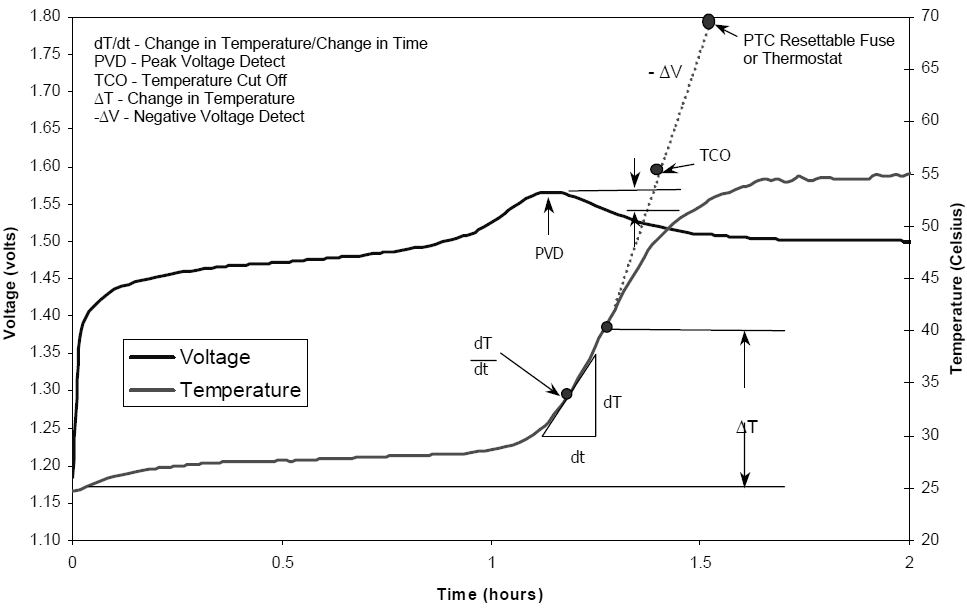
\includegraphics[angle=0,width=14cm]{LatexBeispiel/Bilder/Ladeschlussbw.png}
\caption{Ladeschlusserkennungen, Harding Battery Handbook\cite{Harding}}
\label{Ladeschluss}
\end{figure}

\newpage
So kann Code eingefügt werden.
\begin{lstlisting}[frame=single,breaklines=true,basicstyle=\tiny,language=C,label={PWMStart},caption={Kommentierter Start der PWM}]
/*! \brief Starts the PWM
 * 
 * To make sure that the PWM behaves correctly after a Compare Bit Change the PWM is started and reset with a software trigger.
 */
static void vStartPwm( void )
{
	tc_start( &AVR32_TC0, PWM_CHANNEL );
	tc_software_trigger( &AVR32_TC0, PWM_CHANNEL );
}
\end{lstlisting}

% !TeX encoding = UTF-8
\chapter[Client]{Client}
\thispagestyle{fancy}
\label{client}

Die Beschreibung des Client bezieht sich im Folgenden nur auf die Applikation, welche Sprecher oder Zuhörer für die Präsentation zur Steuerung und Ansicht auf ihrem Endgerät benutzen. Client meint in diesem Zusammenhang nicht den vom Server gesteuerten Projektor.

\section[Grafische Benutzeroberfläche (GUI)]{Grafische Benutzeroberfläche (GUI)\footnote{Sascha Brexeler}}
\label{GUI}
Die Gestaltung dieser GUI bezweckt eine leicht verständliche intuitiv bedienbare Oberfläche mit zielführender Benutzerführung und Hilfestellungen.
Die GUI ist für Geräte mit Android als Betriebssystem entwickelt, aber theoretisch nach dem kompilieren mit eventuell erforderlichen kleinen Anpassung auch auf andere Plattformen/Geräten ähnlich abgebildet und verwendbar. Erfolgreich getestet ist die App allerdings derzeit nur für Android (4.3 + 4.4) und Windows.


\begin{figure}[ht!]
	\centering
	\begin{minipage}{0.31\linewidth}
		\centering
		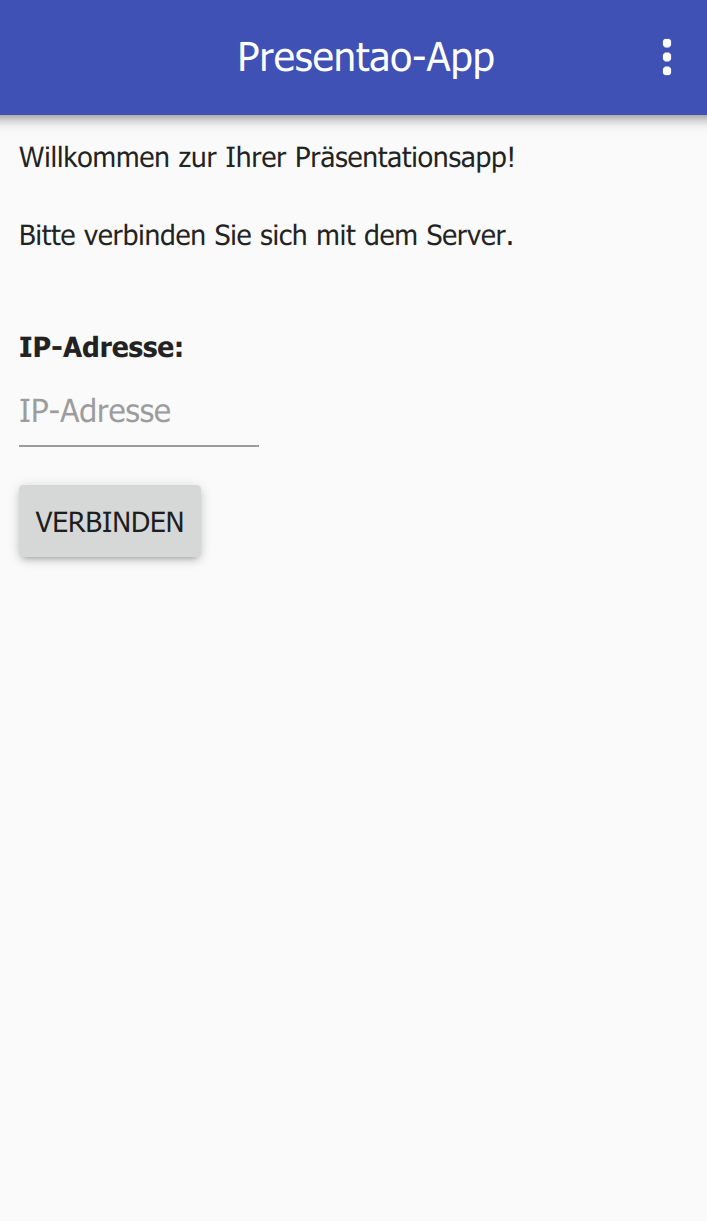
\includegraphics[scale=0.5]{GUI/Bilder/1-Startbildschirm.PNG}
	\end{minipage}
	%\hfill
	\begin{minipage}{0.31\linewidth}
		\centering
		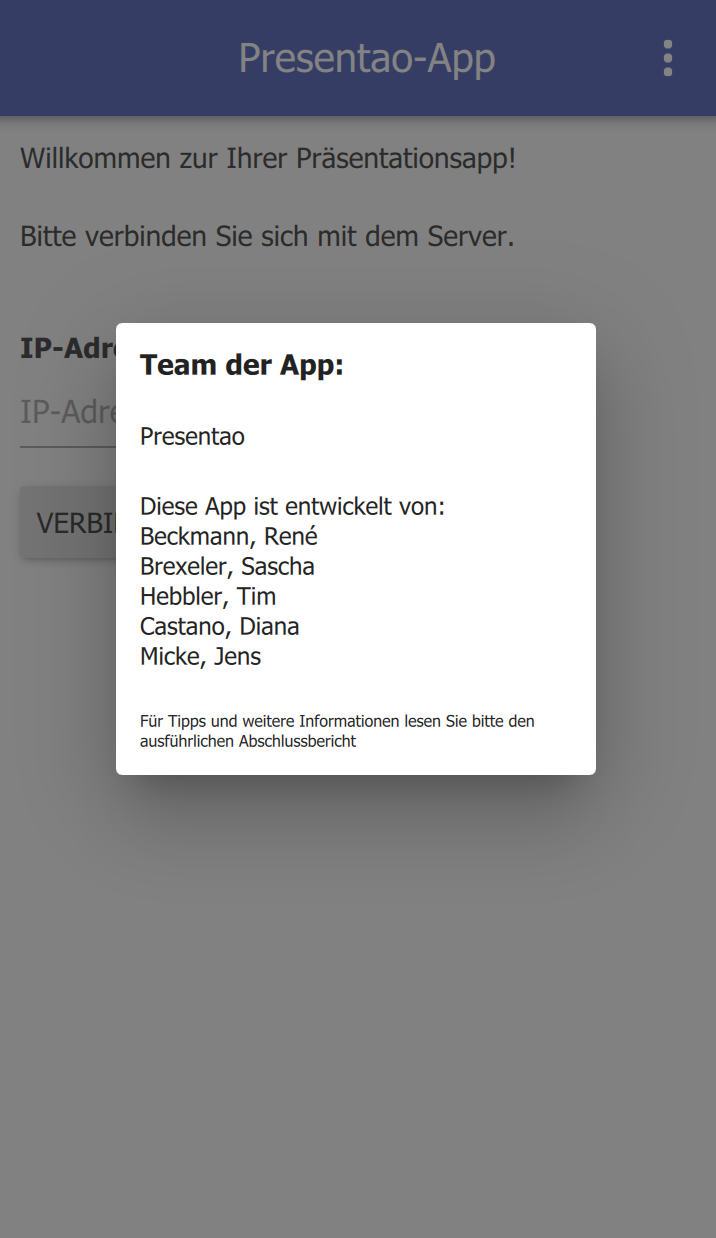
\includegraphics[scale=0.5]{GUI/Bilder/1-0-1-Startbildschirm-PopUP-Team.PNG}
	\end{minipage}
	\begin{minipage}{0.31\linewidth}
		\centering
		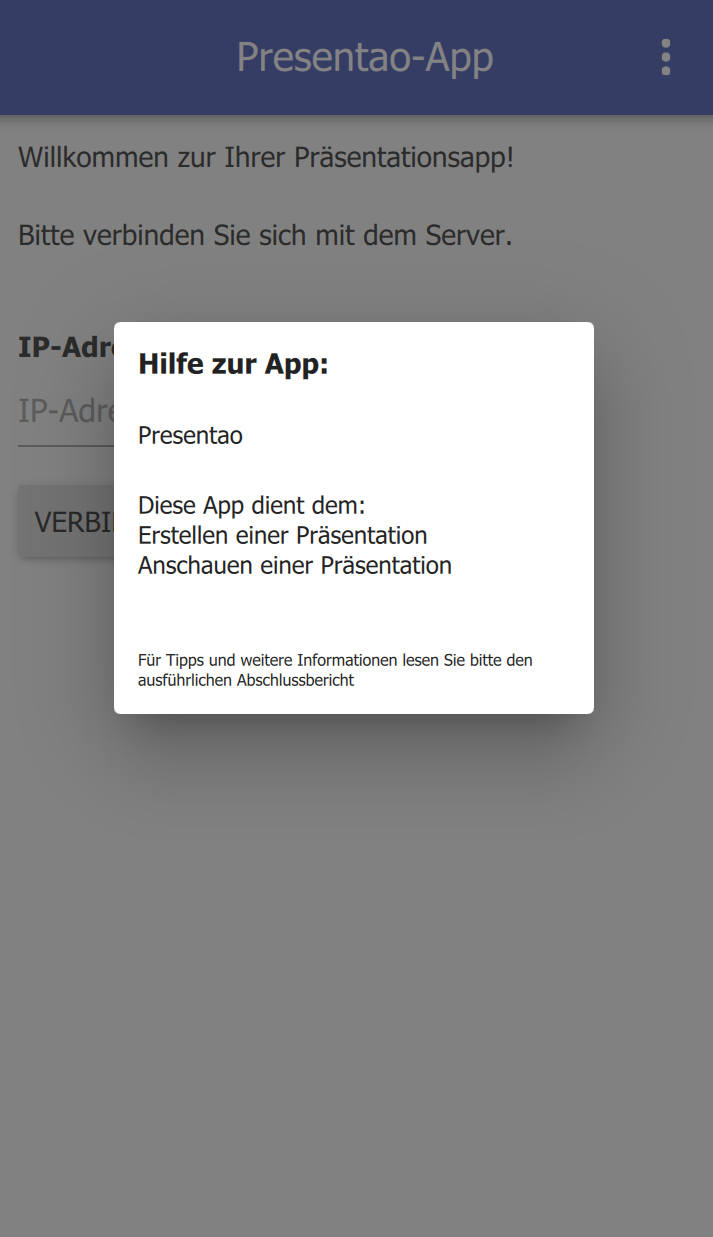
\includegraphics[scale=0.5]{GUI/Bilder/1-0-1-Startbildschirm-PopUP-Hilfe.PNG}
	\end{minipage}
	\caption{v.l.n.r.: Startbildschirm, Über die App, Hilfemenü{\tiny}}
	\label{client:Appstart}
\end{figure}

\newpage

\paragraph{Start der App}$\;$\\
Von dem Startbildschirm aus besteht die Möglichkeit ein Menü (siehe \autoref{client:OptionsMenue}) durch klicken auf den aus drei Punkten bestehenden Menü-Button (siehe \autoref{client:Appstart}) aufzurufen.
\\In diesem lassen sich zwei Pop-Ups zur Hilfe und zum Team aufrufen (siehe \autoref{client:Appstart}).
\begin{figure}[ht!]
	\centering
	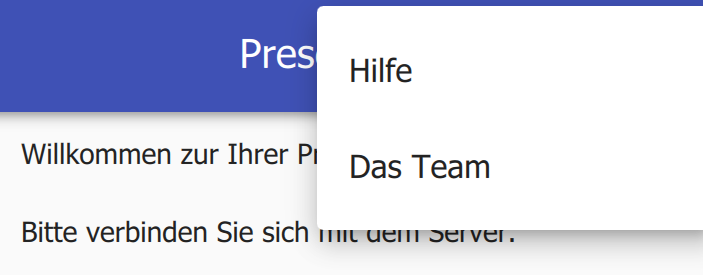
\includegraphics[scale=0.5]{GUI/Bilder/Info-Menu.PNG}
	\caption{Menü{\tiny}}
	\label{client:OptionsMenue}
\end{figure}
\paragraph{Verbindungsaufbau}$\;$\\
Des Weiteren kann der Benutzer nach Eingabe einer der gültigen IP-Adresse eine Verbindung zum Server als Zuhörer aufbauen. Die Eingabe der IP-Adresse erfolgt, wie in der üblichen Notation, mit Punkttrennung und eine Portangabe ist nicht nötig, da diese in Client und Server fest einprogrammiert ist.

\begin{figure}[ht!]
	\centering
	\begin{minipage}{0.31\linewidth}
		\centering
		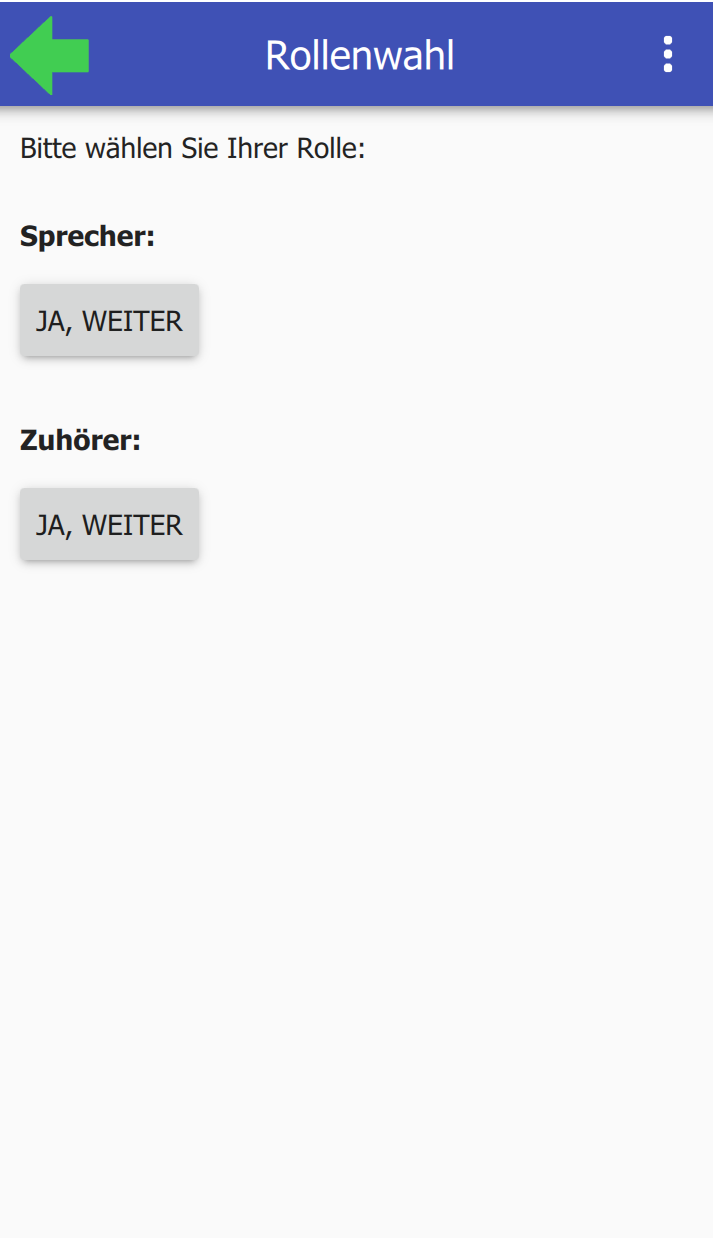
\includegraphics[scale=0.5]{GUI/Bilder/2-Rollenwahl.PNG}
	\end{minipage}
	%\hfill
	\begin{minipage}{0.31\linewidth}
		\centering
		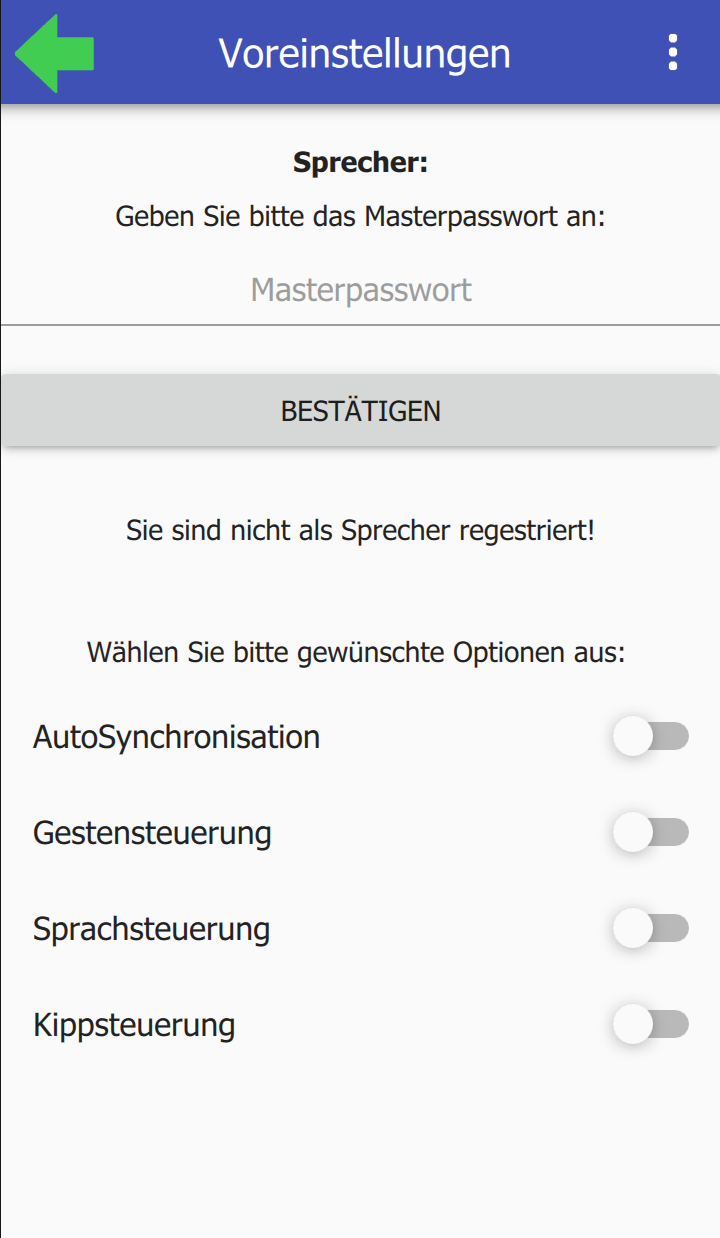
\includegraphics[scale=0.5]{GUI/Bilder/3-S-1-Voreinstellung.PNG}
	\end{minipage}
	\begin{minipage}{0.31\linewidth}
		\centering
		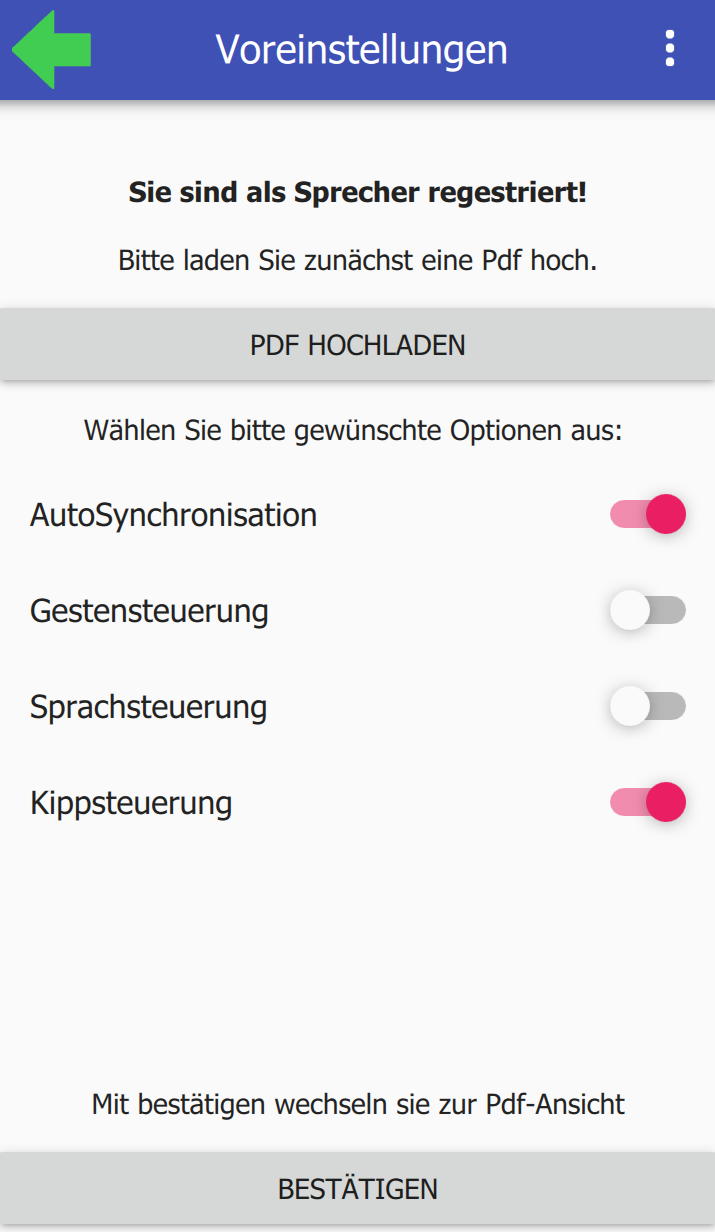
\includegraphics[scale=0.5]{GUI/Bilder/3-S-5-Voreinstellung.PNG}
	\end{minipage}
	\caption{v.l.n.r.: Rollenwahl, Voreinstellungen des Sprecher vor und nach Registrierung{\tiny}}
	\label{client:Rollenauswahl+S-Voreinstellungen}
\end{figure}

\newpage

\paragraph{Auswählen der eigenen Rolle}$\;$\\
Nach erfolgreichen Verbindungsaufbau wechselt die Ansicht in zur Rollenauswahl. Ein Label zeigt diese Position mittig der oberen Leiste (Toolbar) an (siehe \autoref{client:Rollenauswahl+S-Voreinstellungen}).
In dieser Toolbar befindet sich nun zusätzlich ein grüner Pfeil nach links, um zur vorherigen Ansicht zu wechseln.
\\Die Rollenwahl ist wiederholbar und somit korrigierbar, aber unumgänglich implementiert, da weitere Einstellung und Möglichkeiten auf dieser Entscheidung aufbauen.
\paragraph{Voreinstellungen als Sprecher}$\;$\\
Der Sprecher muss sich zunächst als solcher bei dem Server registrieren. Dazu ist eine Passwortabfrage eingerichtet. Das sog. Masterpasswort ist "`mpw12345"'. Wenn die Eingabe fehlerhaft erfolgte, erscheint zusätzlich unter dem Textfeld zur Passworteingabe (siehe \autoref{client:Rollenauswahl+S-Voreinstellungen}) in Dickschrift der Hinweis: "`Bitte überprüfen Sie Ihre Passworteingabe"'. Sobald die Eingabe richtig und bestätigt ist, kann der Benutzer eine Pdf-hochgeladen. Dazu muss der Nutzer eine Pdf-Datei über den File-Dialog (siehe \autoref{client:FileDialog}) suchen und auswählen. Eine Erfolgreiche Auswahl sendet die Datei an den Server, der diese direkt an über den Projektor auf Seite 0 ausgibt. Bevor der Sprecher mit Bestätigen zur Pdf-Ansicht wechselt, sieht dieser noch eine Liste (ListView) mit einige Optionen aus denen er gewünschte über Schiebeschalter (SwitchDelegates) auswählen kann. Mit dem grünen Pfeil wechselt die Ansicht diesmal zurück zur Rollenwahl.

\begin{figure}[ht!]
	\centering
	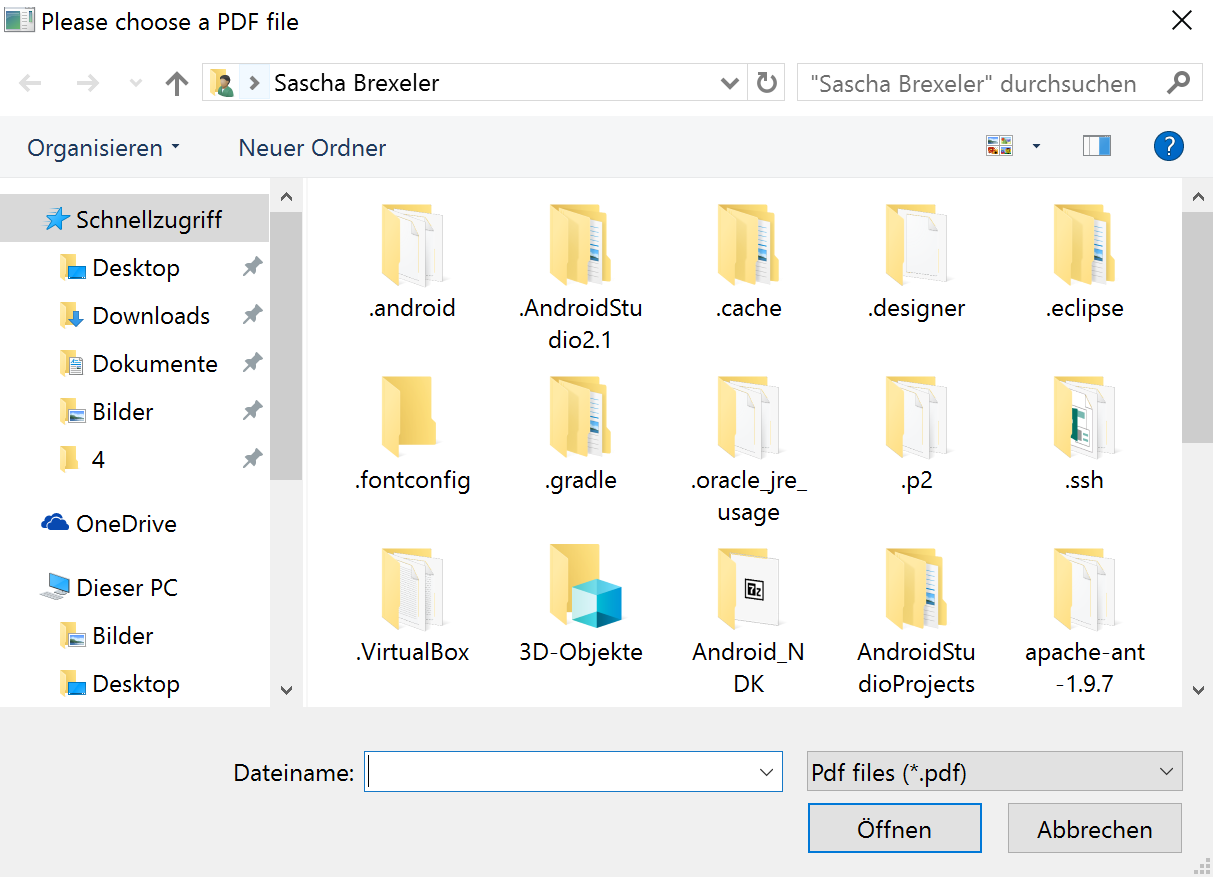
\includegraphics[scale=0.7]{GUI/Bilder/3-S-4-Voreinstellung.PNG}
	\caption{File-Dialog{\tiny}}
	\label{client:FileDialog}
\end{figure}

\begin{figure}[ht!]
	\centering
	\begin{minipage}{0.31\linewidth}
		\centering
		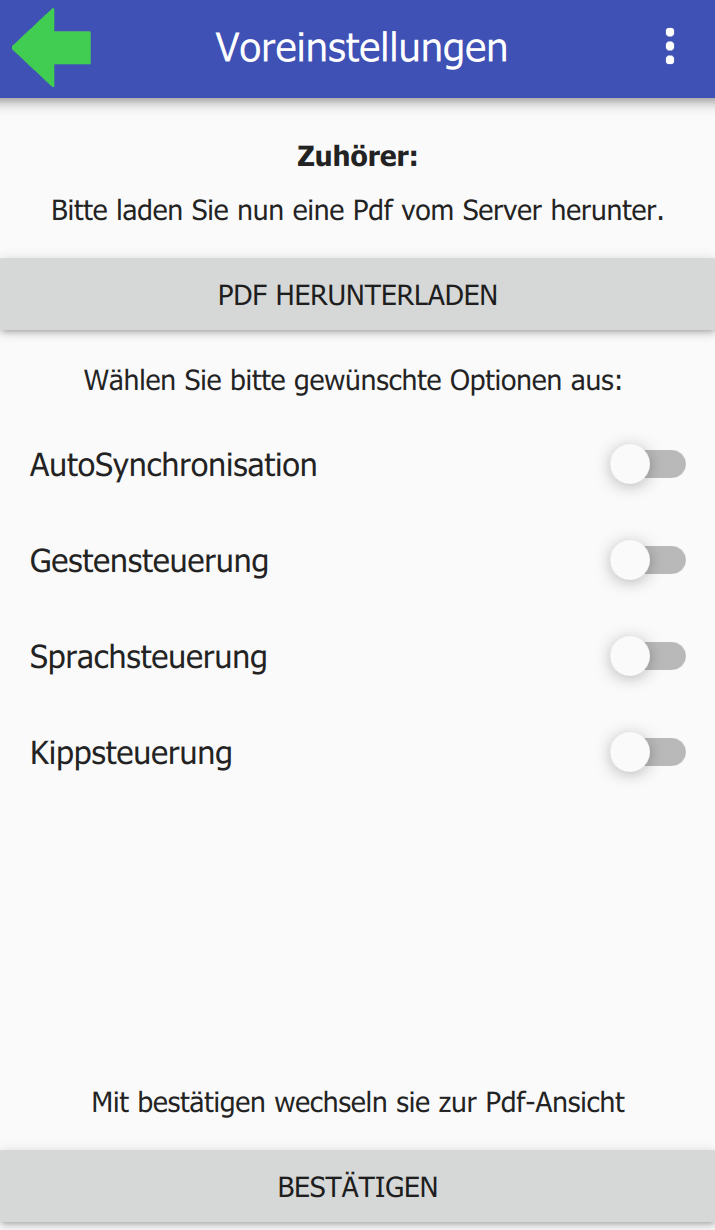
\includegraphics[scale=0.5]{GUI/Bilder/7-H-Voreinstellungen.PNG}
	\end{minipage}
	%\hfill
	\begin{minipage}{0.31\linewidth}
		\centering
		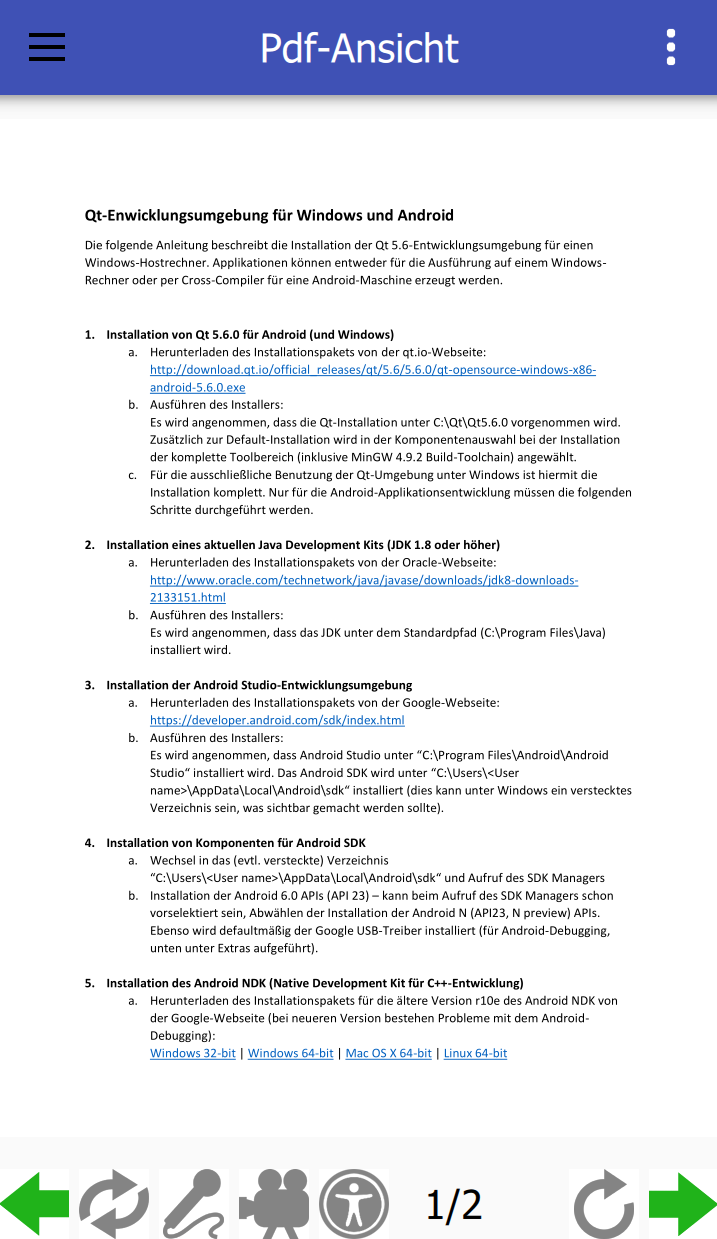
\includegraphics[scale=0.5]{GUI/Bilder/4-S-PDF-Ansicht.PNG}
	\end{minipage}
	\begin{minipage}{0.31\linewidth}
		\centering
		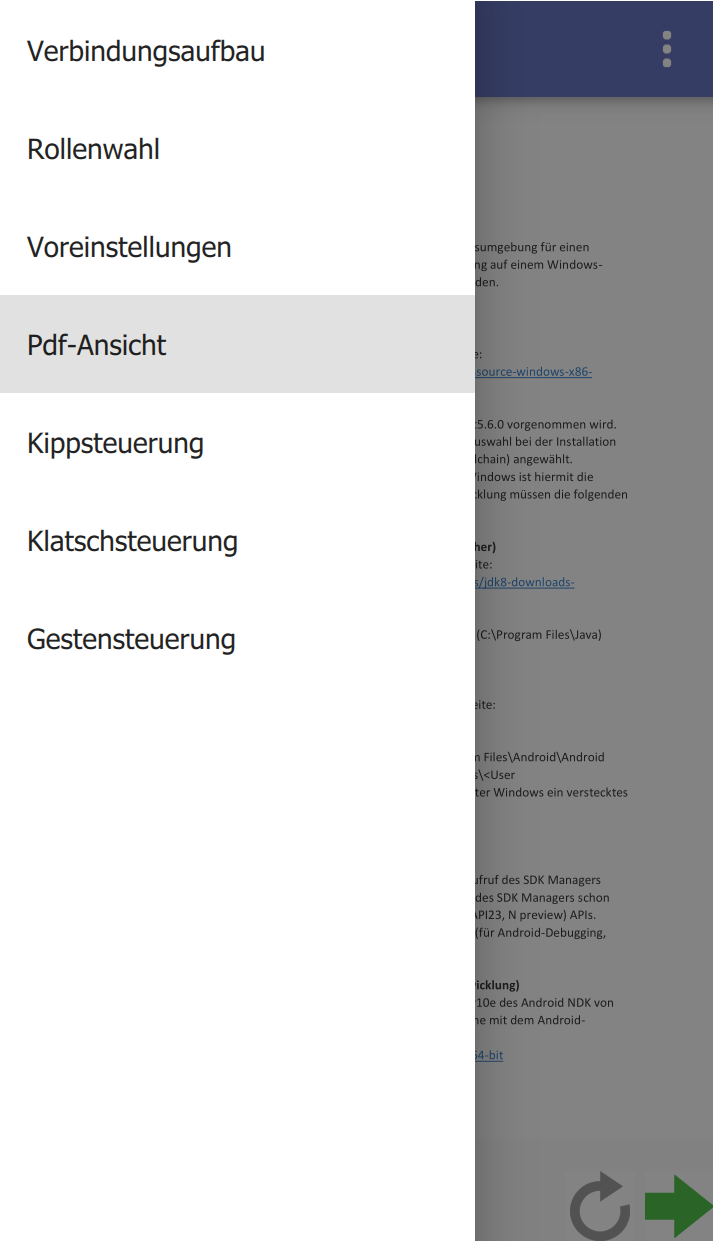
\includegraphics[scale=0.5]{GUI/Bilder/6-Menu-Button-Drawer-mit-Listview.PNG}
	\end{minipage}
	\caption{v.l.n.r.: Voreinstellungen des Zuhörers, PdfAnsicht und Drawer{\tiny}}
	\label{client:H-VoreinstellungenPdfAnsichtDrawer}
\end{figure}

\newpage

\paragraph{Voreinstellungen als Zuhörer}$\;$\\
Als Zuhörer sind die Voreinstellungen ähnlich, jedoch entfällt die Passworteingabe und Herunterladen einer Pdf-Datei ersetzt den Vorgang des Hochladens (siehe \autoref{client:H-VoreinstellungenPdfAnsichtDrawer}). Hierbei erfolgt (ohne eine Auswahlmöglichkeit) das Herunterladen der zuletzt auf dem Server geladenen Datei.
\paragraph{Pdf-Ansicht}$\;$\\
Bestätigen der Voreinstellungen des Sprechers oder Zuhörers bedingt einen Kontextwechsel zur Pdf-Ansicht (siehe \autoref{client:H-VoreinstellungenPdfAnsichtDrawer}).
\paragraph{Drawer}$\;$\\
Ab der Pdf-Ansicht ist der grüne Pfeil oben links durch einen weiteren aus drei waagerechten Strichen bestehenden Menü-Button ersetzt. Dieser Button öffnet eine vertikale Leiste (Drawer) am linken Bildschirmrand, welche ein ListView beinhaltet, dass schnelle Navigation zu allen bisherigen Ansichten und Weiteren ermöglicht (siehe \autoref{client:H-VoreinstellungenPdfAnsichtDrawer}). Durch wischen am vom linken Bildschirmrand nach rechts lässt sich dieser ebenfalls einblenden. Die Navigation über das ListView im Drawer ist nur möglich solange man nicht zu vorherigen Ansichten wechselt. 
\paragraph{Symbolleiste}$\;$\\
Die Pdf-Ansicht beinhaltet ein Symbolleiste (siehe \autoref{client:Symbolleiste}) als Reihe von Icons am unteren Bildschirmrand. Mit ihr ist durch die Pfeile außen ein Blättern in der Pdf möglich. Intuitiv blättert der linke Pfeil zurück, der Rechte vor. Die anderen Buttons dienen dem aktivieren/deaktivieren von Bedienoptionen. Grün signalisiert hierbei aktiviert und grau deaktiviert. Das Mikrofon steht für die Audiosteuerung, das Kamerasymbol für  Gestensteuerung und das Männchen mit den ausgestreckten Armen und Beinen im Kreis für die Kippsteurung. Neben diesem Symbol steht die Seitennummer der angezeigten Seite.
\\Die ineinander greifenden Pfeile signalisieren bei grün, dass die Autosynchronisation aktiv ist. Sobald diese nicht aktiv ist, erscheint ein weiterer Pfeil geschlungen im Uhrzeigersinn in grau auf der Symbolleiste links neben dem Pfeil. Die Funktion ist das manuelle Aktualisieren der Seitenzahl. Ein Sprecher sendet mit dem Refresh-Button die Seitenzahl, die auf seinem Device aktuell ist zum Server, und dieser leitet sie an die Zuhörer-Clients weiter. Ist als Sprecher Autosynchronisation aktiviert, geschieht die bei jedem Blättern automatisch. Zuhörer können über Refresh die aktuelle Seite manuell anfragen oder mit Autosynchronisation alle 2 Sekunden zu der aktuellen Seite zurück springen. Wenn der Sprecher Blättert, erhalten die Zuhörer jedoch in jedem Fall die aktuelle Seite.

\begin{figure}[ht!]
	\centering
	
\includegraphics[scale=0.5]{GUI/Bilder/SchnellLeiste.PNG}
	\caption{Symbolleiste{\tiny}}
	\label{client:Symbolleiste}
\end{figure}

\paragraph{Informationen zur Benutzung}$\;$\\
Da das bisherige Hilfe-Pop-Up nur recht allgemeine Informationen enthält sowie für weitere Hilfestellung auf diese eventuell nicht zur Hand liegenden Dokumentation verweist, kann sich der Benutzer über den Drawer zu einer Erklärung der Bedienmöglichkeiten navigieren. Diese Möglichkeit soll einen möglichst einfachen Einstieg ohne viel ausprobieren sicherstellen und Anwendungsfehler verhindern. Um einen mit dieser Anwendung vertrauten Anwender nicht nach jedem Start durch diese Informationen zu führen, ist das Aufrufen optional (siehe \autoref{client:Symbolleiste}).

\begin{figure}[ht!]
	\centering
	\begin{minipage}{0.31\linewidth}
		\centering
		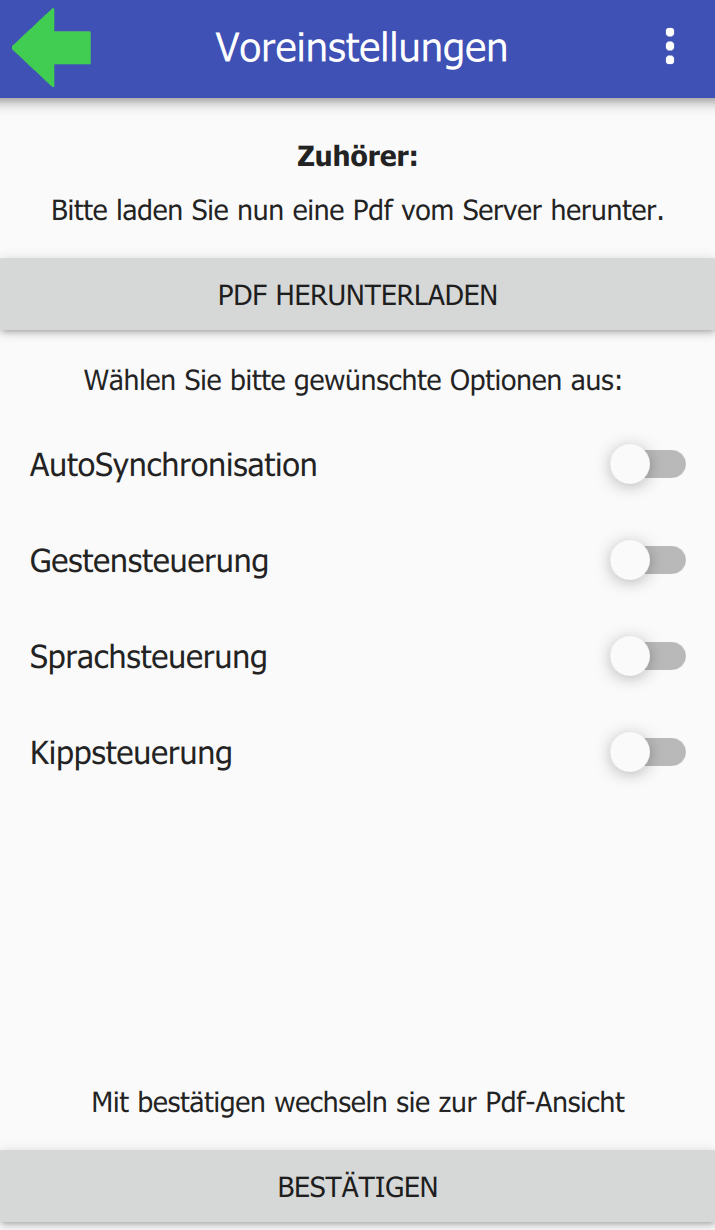
\includegraphics[scale=0.5]{GUI/Bilder/7-H-Voreinstellungen.PNG}
	\end{minipage}
	%\hfill
	\begin{minipage}{0.31\linewidth}
		\centering
		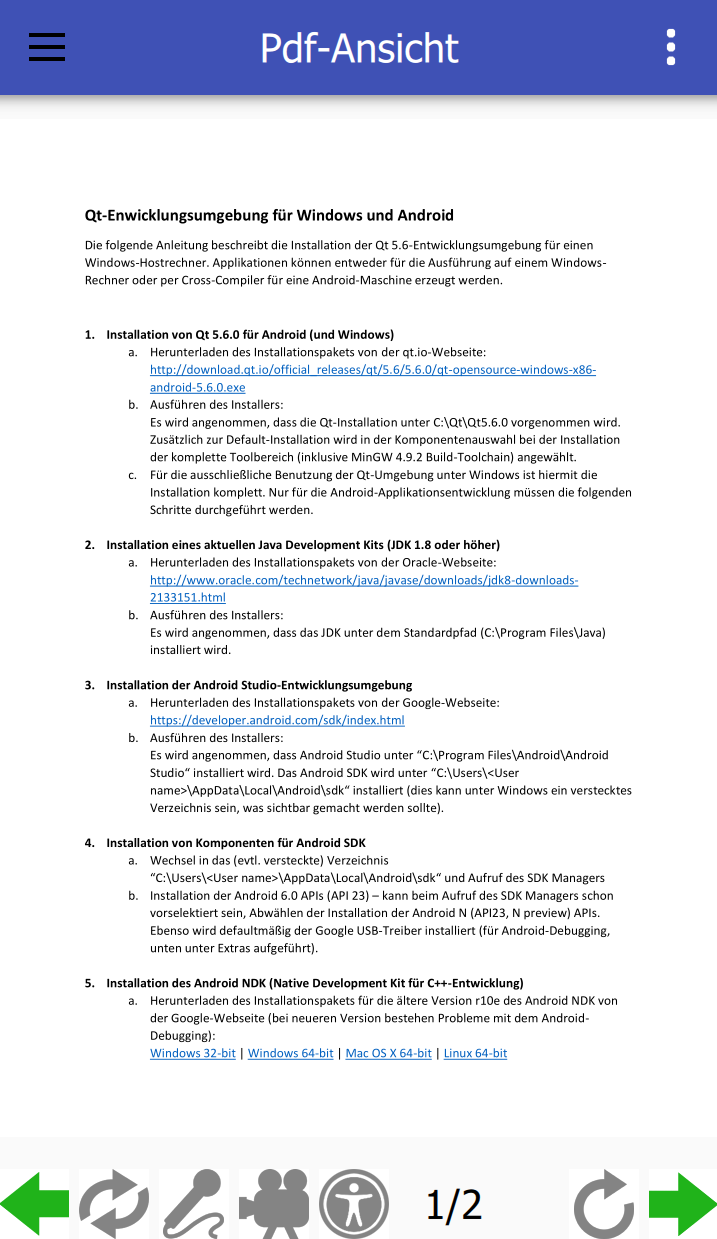
\includegraphics[scale=0.5]{GUI/Bilder/4-S-PDF-Ansicht.PNG}
	\end{minipage}
	\begin{minipage}{0.31\linewidth}
		\centering
		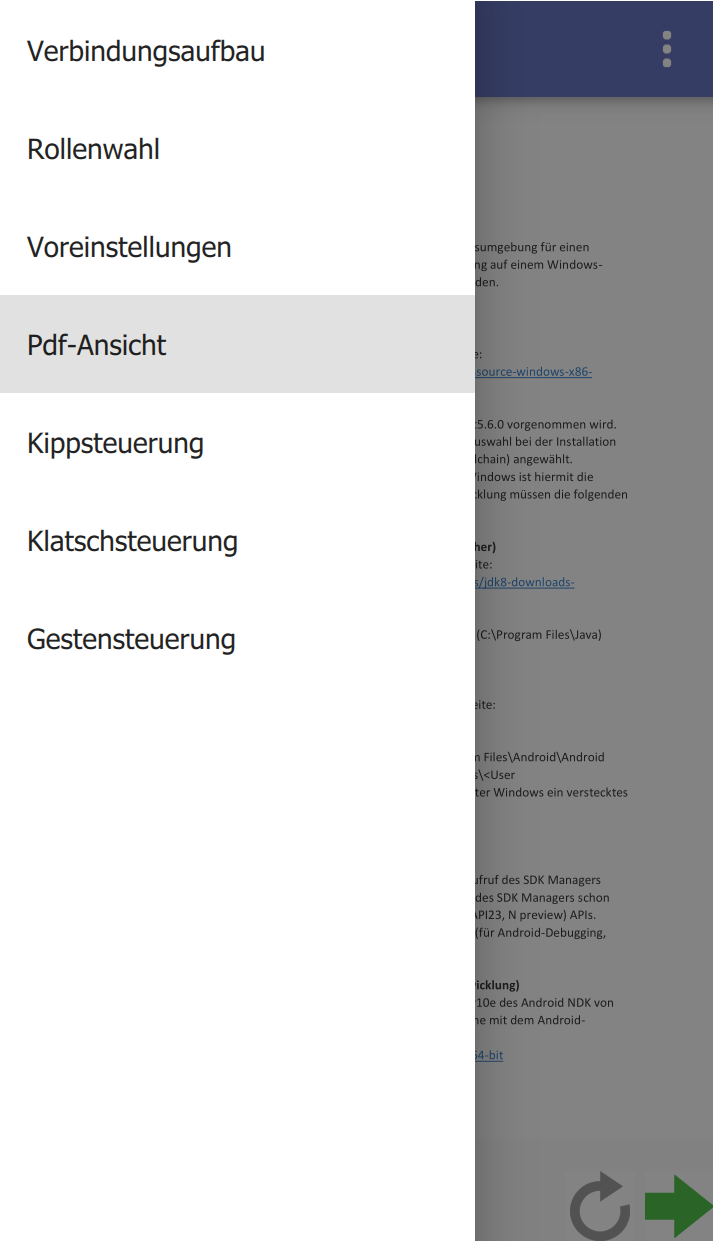
\includegraphics[scale=0.5]{GUI/Bilder/6-Menu-Button-Drawer-mit-Listview.PNG}
	\end{minipage}
	\caption{v.l.n.r.: Gestensteuerung, Kippsteuerung und Klatschsteuerung{\tiny}}
	\label{client:InformationenBedienhilfen}
\end{figure}


\section[Serveranbindung]{Serveranbindung\footnote{Sascha Brexeler}}
\label{client-Serveranbindung}
Die Einbindung der Funktionsblöcke zur Kommunikation des Clients mit dem Server ist in Zusammenarbeit\footnote{zwischen Sascha Brexeler und René Beckmann} im Team entstanden. Hier erfolgt nur eine grobe Beschreibung. Details zur Kommunikation finden Sie in Kapitel ????


\section[Software]{Software\footnote{Sascha Brexeler}}
\label{guiSoftware}
Die Software finden Sie im Git Repository  \footnote{https://github.com/BeckmaR/EmbeddedMultimediaSS2016/tree/master/src/} in im Ordner


\paragraph{Konzept}$\;$\\
Das Softwarekonzept dient der Umsetzung des Bedienkonzepts mit "Qt-Creator"' programmiert in C++ und Qml. Der Qt-Creator ist dafür wegen der Plattformunabhängigkeit ausgewählt.
\paragraph{Struktur}$\;$\\

\paragraph{Zustandssteuerung}$\;$\\
Die Realisierung der Grafische Oberflächen entsprechend bisheriger Einstellungen ist über Zustände einer Variablen "`appState"' realisiert, die sich die aktuellen Einstellungen bzw. den Ort merkt und entsprechend Informationen mittels der Objekteigenschaft "`visible"' ein oder ausblendet.
\paragraph{Elemente}$\;$\\
\paragraph{Einbindung der erweiterten Bedienmöglichkeiten}$\;$\\
\paragraph{Details}$\;$\\
\paragraph{Lektionen}$\;$\\

\section{Navigation}
% !TeX encoding = UTF-8
\chapter{Gestensteuerung}
\thispagestyle{fancy}

Die Gestensteuerung hat die Aufgabe Handbewegungen über eine Smartphone-Kamera zu erkennen. Dabei werden zwei Richtungen erkannt und Signale zum vor- und zurückblättert von PDF-Seiten gesendet. Auf Grund der Vorlesung und Recherchen im Internet war schnell klar, dass \href{http://opencv.org/}{OpenCV} eine zweckmäßige Bibliothek darstellt. Als Qt Basis wurde die Version 5.7 und OpenCV in der Version 3.1 verwendet. Der Code für die Gestenerkennung befindet sich unter folgendem \href{https://github.com/BeckmaR/EmbeddedMultimediaSS2016/tree/master/src/handcontrol}{Link}. Hierbei wurde ein C++ Klasse "`handcontrol"' erstellt, welche in die App eingebunden ist.

\section{Auslesen von Videoframes aus einer Kamera}
Im Laufe des Projektes stellte sich heraus, dass die Einbindung der Kamera, auf den verschiedenen Plattformen Windows und Android, die größte Herausforderung darstellt. Die Windows Unterstützung wurde hauptsächlich ausgewählt, um den Algorithmus nicht umständlich auf einem Android Gerät jedes mal testen zu müssen. Die Implementierung auf der Windows-Plattform war relativ einfach, da OpenCV schon eine Funktion \href{http://docs.opencv.org/3.1.0/d8/dfe/classcv_1_1VideoCapture.html}{VideoCapture} bietet, welche einzelne Videoframes aus eine Kamera auslesen kann und diese in einer Matrix abspeichert. Diese Methode funktionierte leider nicht auf einen Android-Gerät. Hinweise: nachfolgende Funktionsweisen beziehen sich auf den Entwicklungsstand vom 20.7.2016, ggf. sind schon Bugs behoben oder neue Möglichkeiten zur Kameraauswertung hinzugekommen. Vom Autor wurden unterschiedlichste Varianten zum Auslesen der Kamera über mehrere Stunden untersucht. Von Qt werden hauptsächlich \href{http://doc.qt.io/qt-5/videooverview.html}{zwei Möglichkeiten} für das Auslesen eines VideoFrames angeboten. \href{http://doc.qt.io/qt-5/qabstractvideosurface.html}{QAbstractVideoSurface} definiert eine abstrakte C++ Klasse welche die Funktion present() beinhaltet, welcher die einzelnen Videoframes nacheinander übergeben werden. Ähnlich verhält es sich mit \href{http://doc.qt.io/qt-5/qvideoprobe.html}{QVideoProbe} wobei man hier die Verbindung über ein Connect() mit Signal und Slot hergestellt werden muss. Eine weitere Möglichkeit besteht seit Qt 5.5 darin, ein Video Filter\footnote{\label{video_filter}https://blog.qt.io/blog/2015/03/20/introducing-video-filters-in-qt-multimedia/} in QML zu verwenden und mit Hilfe der Klasse \href{http://doc.qt.io/qt-5/qabstractvideofilter.html}{QAbstractVideoFilter} die einzelnen Videoframes in C++ zu analysieren und ggf. wieder nach QML zu transformieren. Die C++ QCamera funktioniert nicht auf Android-Geräten (\href{https://bugreports.qt.io/browse/QTBUG-41194}{1},\href{http://stackoverflow.com/questions/28041741/qt-qml-camera-to-c-qimage-on-android}{2}), sodass auf das in QML integrierte Camera Objekt zurückgegriffen wird. Bei der QAbstractVideoFiler Variante konnten die Videodaten in Android nicht in den CPU-Adressraum gemappt werden. Mit QVideoProbe war dies möglich. Hierbei wird aus QML das QCamera Objekt in C++ adressierbar gemacht und mit dem QVideoProbe verbunden. Seit Qt 5.6 existiert ein VideoOutput Objekt in QML welches das Auslesen und Anzeigen von VideoFrames steuert, sodass das hier angegebene \href{http://stackoverflow.com/questions/28041741/qt-qml-camera-to-c-qimage-on-android/33238150\#33238150}{Beispiel} noch um ein VideoOutput Objekt ergänzt werden muss. Um keine größeren Unterschiede zwischen dem Algorithmus für die Windows- und der Androidversion zu haben, ist es wünschenswert beide Cameras über Qt auslesen zu lassen. Leider funktioniert der oben für Android vorgestellte Ansatz für Windows nicht. Hier ist ein Workaround mit einer C++ QCamera und dem QAbstractVideoSurface nötig, um ein QVideoFrame zu erhalten. Die neue Variante mit dem "`Video Filter"' wurde auch untersucht, hat aber nur auf ein paar Androidgeräten funktioniert \href{https://bugreports.qt.io/browse/QTBUG-47934/}{QTBUG-47934}. Anscheinend gibt es dort noch Fehler in dem Qt-Framework. Unter folgendem \href{https://wiki.qt.io/Qt_5.7_Multimedia_Backends}{Link} gibt es eine Auflistung welche Funktionen in dem Qt-Multimedia-Framework-5.7 auf den verschiedenen Plattformen aktuell funktionieren.

\subsection{Verbesserungen}
Die mit Qt 5.5 eingeführten Video Filter scheinen ein gute Weg zu sein, um VideoFrames in Qt analysieren zu können. Leider ist aktuell die Implementierung nicht auf allen Androidgeräten funktional, sodass auf ein Workaround mit QVideoProbe zurückgegriffen werden musste. Diese Variante ist aber leider nicht optimal, da sie Verzögerungen zwischen dem Aufnehmen und dem Aufruf der Funktion present() enthält\footnote{https://blog.qt.io/blog/2015/03/20/introducing-video-filters-in-qt-multimedia/\#comment-1195419}. Eine weitere Möglichkeit besteht, QML \href{http://doc.qt.io/qt-5/qml-qtquick-shadereffect.html}{ShaderEffect} mit OpenGL zu verwenden. Da die Android Kamera seine Videoframes auf der Grafikkarte in OpenGL Texture vorhält \footnote{https://blog.qt.io/blog/2015/03/20/introducing-video-filters-in-qt-multimedia/\#comment-1195414}, wäre es sinnvoll diese auch dort weiter zu verarbeiten. Das kann seit neuem mit Video Shader Objekten direkt in QML programmiert werden. Außerdem war es dem Autor über QML nicht möglich exakte Auflösungen und Frameraten einzustellen. Anscheinend ignoriert Qt gewisse Parameter auf verschiedenen Platformen oder es stehen nicht alle Einstellung zur Verfügung. Jedenfalls sind diese nicht richtig dokumentiert. Ein Problem ist außerdem, dass es vorkommen kann das Frameraten von 30 fps auf 16 fps einbrechen oder kein reproduzierbares Verhalten zeigen. Dieser Punkt konnte innerhalb der Arbeit leider nicht geklärt werden. Eine andere Möglichkeit, welche nicht weiter verfolgt wurde, wäre über Qt mit den \href{http://doc.qt.io/qt-5/qtandroidextras-module.html}{Qt Android Extras} die Androidkamera über Java Code in die Qt Anwendung einzubetten, ggf. auch über das vorhandene OpenCV Java Binding. 

\section{Handerkennungsalgorithmus}
Aus Qt liegen die QVideoFrames als RGB (Windows) und als YUV420 (Android) vor. Diese werden als erstes in Grauwertbilder umgewandelt. Bei dem Android QVideoFrame muss keine pixelweise Konvertierung durchgeführt werden, sondern es wird nur der Luminanz Y Teil des Bildes genommen. Anschließend wird das Differenzbild zwischen dem aktuellen und vorherigen Grauwertbild berechnet. Hierbei achtet OpenCV selbständig darauf, dass eine Sättigung im Zahlenbereich durchgeführt wird.

\begin{figure}[ht!]
\centering
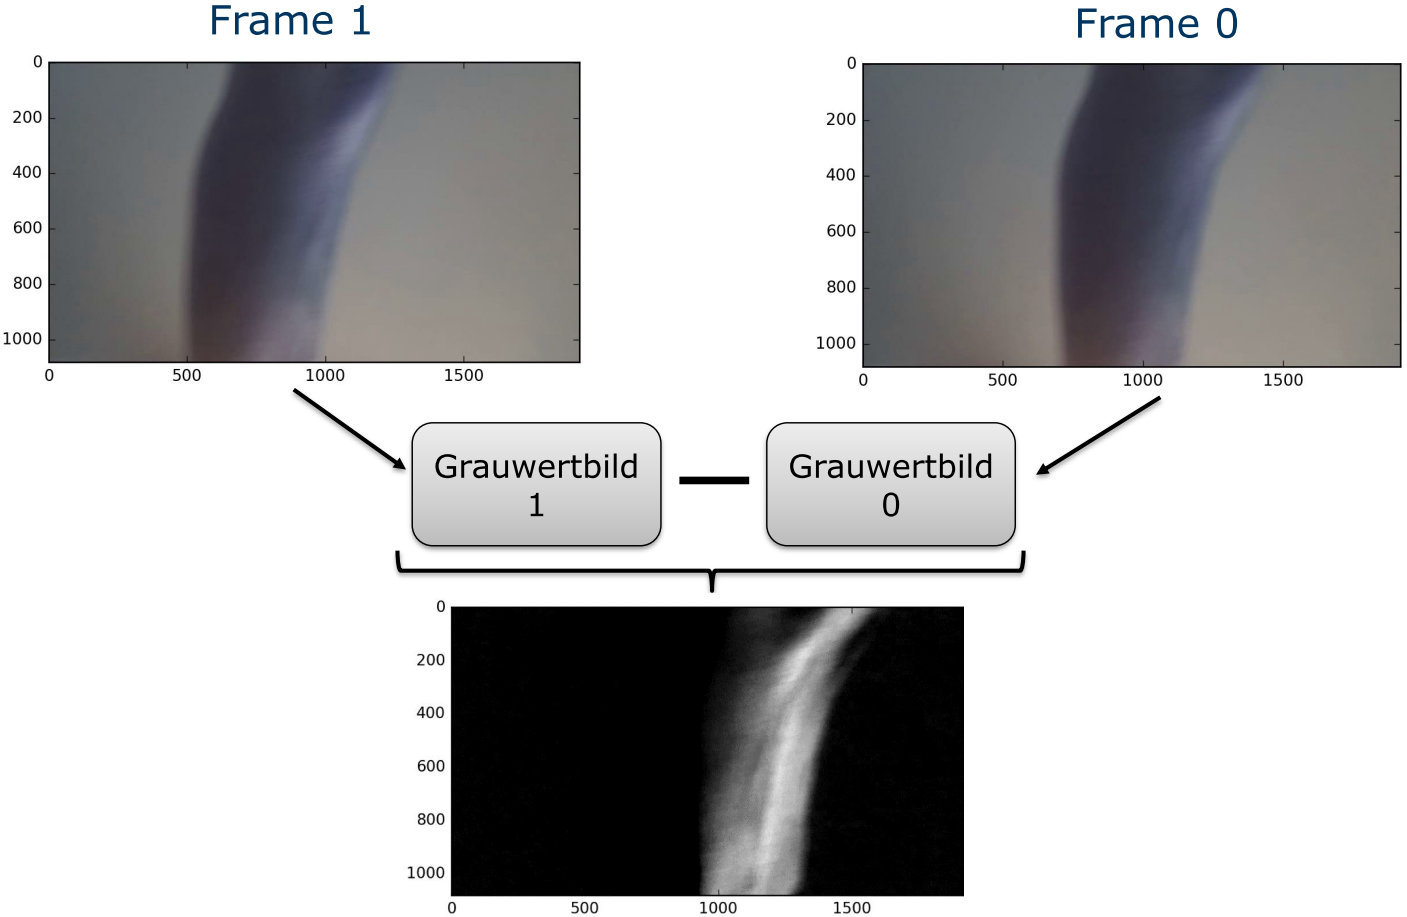
\includegraphics[angle=0,width=14cm]{handcontrol/Bilder/diff_frame1-frame0.png}
\caption{Differenzberechnung zwischen aktuellem und vorherigen Grauwertbild}
\end{figure}

Im nachfolgenden Schritt wir mit Hilfe der reduce() Funktion von OpenCV ein Mittelwert über alle Spalten gebildet. Man erhält einen Zeilenvektor wobei jeder Eintrag den Mittelwert eine Spalte repräsentiert. Hierbei kann man schnell erkennen wo sich in der Horizontalen die größten Änderungen ergeben. Das nennt der Autor Histogramm, da es die Häufigkeitsverteilung darstellt.

\begin{figure}[ht!]
\centering
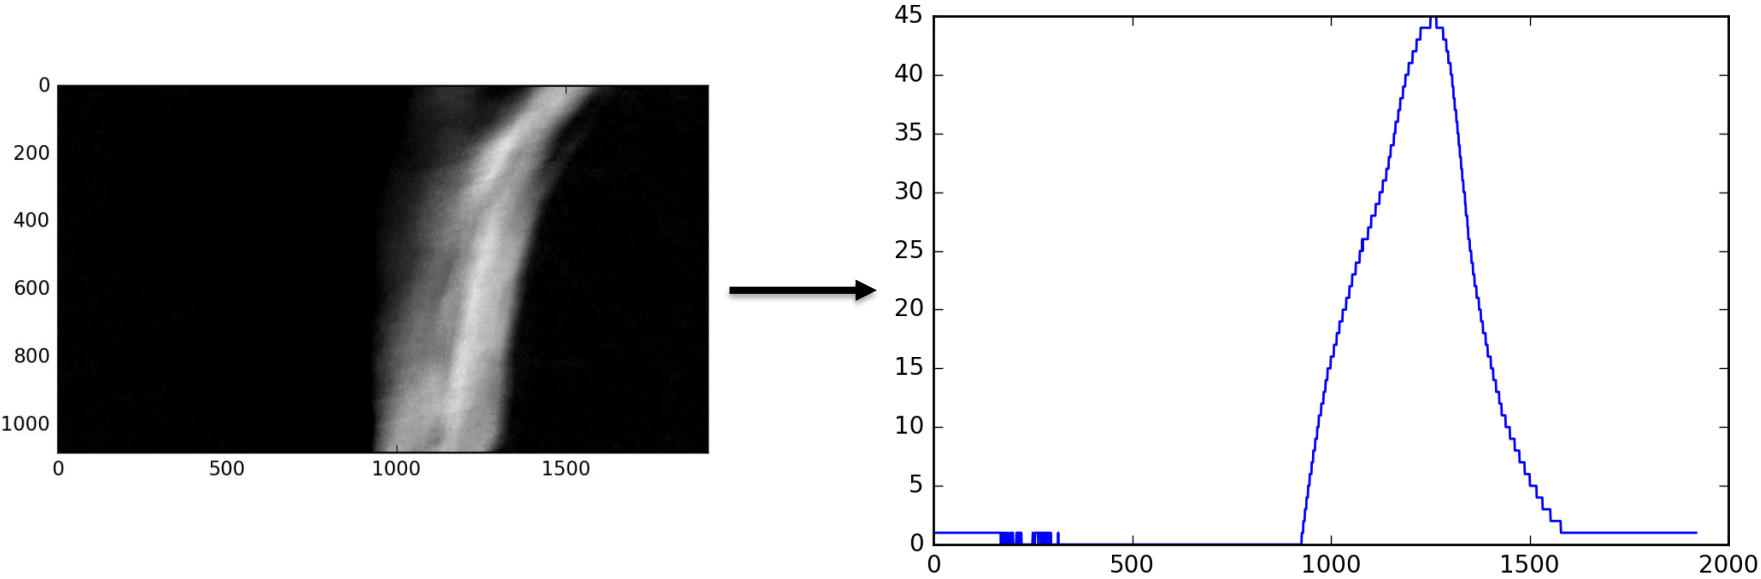
\includegraphics[angle=0,width=14cm]{handcontrol/Bilder/diff_frame_to_hist.png}
\caption{Berechnung des Histogramms über die Spalten eines Differenzbildes}
\end{figure}

Untersucht man die Verschiebung des Histogramms über die Horizontalen, kann man Handbewegungen erkennen. Hierbei wird als erstes der Schwerpunkt des Histogramms gebildet. Das geschieht mit Hilfe einer kumulierten Summe über alle Histogrammwerte. Würde man nur den maximalen Wert des Histogramms betrachten, kann bei verrauschten Bildern eine zu große Abweichung auftreten. Vor dem Berechnen des Schwerpunktes wird noch ein konstanter Faktor subtrahiert, um den ggf. existierenden Rauschteppich zu entfernen. Zur weiteren Fehlerreduktion wurden im folgenden nur diese Schwerpunkte ausgewählt, welche auch mindestens einen gewissen maximalen Histogrammwert aufweisen. Der Wert kann im Sourcecode nachgelesen werden. Um auszuwerten, ob eine PDF vor- oder zurückgeblättert werden soll, untersucht der Algorithmus zeitlich aufeinanderfolgende Schwerpunkte von Histogrammen der Differenzbilder. Er sendet ein Signal, wenn ohne Unterbrechung der Schwerpunkt eine gewisse Zeit in eine der beiden Richtungen gewandert ist. Um den GUI-Thread nicht zu überlasten und um eine flüssige Bedienung der GUI sicher zu stellen, wurde der Algorithmus in ein QThread verschoben. Der so beschriebene Algorithmus benötigt mit 30 Frames pro Sekunde auf Windows ~7ms und auf Android ~10 ms. Somit ist die Echtzeitfähigkeit gegeben. Als Alternative zum dem Differenzbild wurde auch der in OpenCV implementierte Background Substraction Algorithmus (\href{http://docs.opencv.org/3.0-rc1/d7/d7b/classcv_1_1BackgroundSubtractorMOG2.html}{BackgroundSubtractorMOG2}) untersucht. Dieser schätzt den Hintergrund über gaußsche Mischungsverhältnisse mit Mittelwert und Kovarianzmatrix. Leider benötigt der Algorithmus viel Berechnungszeit (~14 Windows und ~30 ms Android) und kratzt somit bei Android Geräten an der Echtzeitfähigkeit. Außerdem würde eine solche Implementierung zu viel Energie des Akkus verbrauchen und wurde deshalb verworfen.

\begin{figure}[ht!]
\centering
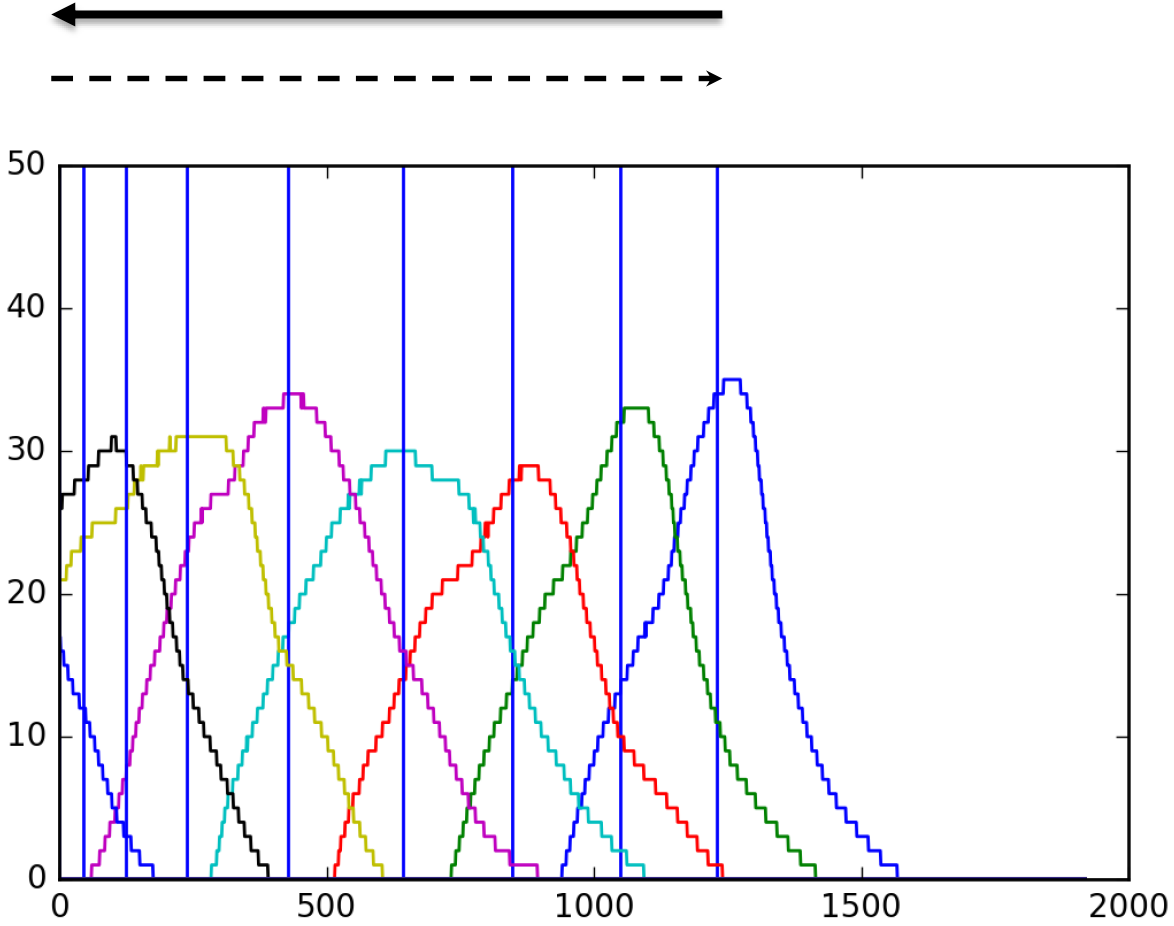
\includegraphics[angle=0,width=14cm]{handcontrol/Bilder/histogramm_schwerpunkt.png}
\caption{Histogramme der Differenzbilder mit Schwerpunkt}
\end{figure}

\section{Entwicklung des Algorithmus}
Der Algorithmus wurde als erstes in MATLAB mit aufgenommenen Videos entwickelt. Nachher wurde auf Python mit OpenCV Binding umgestellt, um einen besseren Vergleich mit der C++ Version zu gewährleisten. Als IDE für Python wurde \href{https://github.com/spyder-ide/spyder}{Spyder} mit dem \href{https://www.continuum.io/downloads}{Anaconda Framework} verwendet. Um den Algorithmus separat von der App zu entwickeln wurde ein "`test\_handcontrol.pro"' Projekt erstellt, welches als eine Art Modultest fungiert. Zu finden in dem schon am Anfang des Kapitels genannten Verzeichnis in Github.

\section{Verbesserungen}
Die Verbesserungen zum Auslesen der Kamera wurden schon in einem separaten Abschnitt behandelt. Für den Algorithmus könnte man statt Grauwertbilder auch Bilder aus dem HSV Raum verwenden. Dort könnte man ggf. Helligkeitsveränderung besser abfangen. Außerdem kann es manchmal vorkommen, dass mehrfach Erkennung erfolgen, diese könnten durch einen Timer abgefangen werden. Eine Verschiebung der Berechnung zur Grafikkarte mittels OpenGL oder OpenCL, wie vorher schon erwähnt, könnte die CPU entlasten und ganz andere Möglichkeiten der Analyse des Frames bieten. Bei der Differenzbildung der Frames entstehen positive und negative Abweichungen, diese könnten in einem verbesserten Algo. separat berücksichtigt werden.


\subsection[Navigation Beschleunigungssensor]{Navigation Beschleunigungssensor\footnote{Jens Helge Micke}}
\thispagestyle{fancy}
\label{Beschleunigungssensor}

\section{Features}
- Blättern in einer Pdf ohne dass ein Update auf dem Server erfolgt\\
\\INOF ans TEAM:Diese Section ist noch nicht fertig
\section{Erweiterungspotential}
Einige zusätzliche Funktionalitäten könnten, den Wert der Applikation für Zuhörer und Sprecher steigern.\\
\\INOF ans TEAM:Diese Section lade ich später hoch
\\INOF ans TEAM:Wenn Ihr die Zuverlässigkeit der Gestensteuerung, Kippsteuerung, Audiosteuerung oder die Sicherheit der Kommunikation noch verbessern wollt, könnt ihr ja wie Tim es in euren Abschnitt einfügen. Hier geht es nur um Erweiterungen der allgemeinen mögliche Funktionalität der Clientapp wie Puplikumsfragen oder sowas.
Erweiterungen für den Sprecher:\\

Erweiterungen für den Zuhörer:\\
- Einstellen der Zeit die vergehen soll bis sich die Applikation synchronisiert\\






\newpage
So kann Code eingefügt werden.
\begin{lstlisting}[frame=single,breaklines=true,basicstyle=\tiny,language=C,label={PWMStart},caption={Kommentierter Start der PWM}]
/*! \brief Starts the PWM
* 
* To make sure that the PWM behaves correctly after a Compare Bit Change the PWM is started and reset with a software trigger.
*/
static void vStartPwm( void )
{
tc_start( &AVR32_TC0, PWM_CHANNEL );
tc_software_trigger( &AVR32_TC0, PWM_CHANNEL );
}
\end{lstlisting}
\chapter{PDF Renderer}
\thispagestyle{fancy}

Kapitel erstellt von Tim Hebbeler
\\
Der PDF-Renderer wurde als separate C++-Klasse entwickelt und ist in die Android App und den Server eingebunden.

Im Laufe der Entwicklung wurden die Bibliotheken \href{https://poppler.freedesktop.org/}{Poppler} und \href{http://mupdf.com/}{MuPDF} untersucht. Das Projekt Poppler ist eine unter der GPL stehende Bibliothek und basiert auf \href{https://de.wikipedia.org/wiki/Xpdf}{Xpdf}. Poppler bietet schon ein Qt-Binding, doch leider liegt der Fokus auf unixartige Betriebssysteme und nicht auf der Plattformunabhängigkeit \footnote{\url{https://de.wikipedia.org/wiki/Poppler}}. Die PDF Darstellung wird aber auf verschiedenen Plattform, wie Android, dem Raspberry Pi und Windows benötigt, deshalb konnte Poppler nicht verwendet werden.
Die Wahl fiel deshalb auf MuPdf von der Firma Artifex Software, Inc. ,welches unter der AGPLv3 steht. Diese Bibliothek bieten kein Qt-Bindung, doch existiert ein von einer Privatperson initiiertes Projekt \href{https://github.com/xiangxw/mupdf-qt}{mupdf-qt}, welches Grundfunktionalitäten mit Qt bietet. Hierbei war ein vergleichsweise einfache Cross-/Kompilierung für die verschiedenen Plattformen möglich.

Die GUI-Oberfläche wurde mit Hilfe von QML erstellt, deshalb ist ein Transfer der PDF-Daten von C++ nach QML nötig. Der Slot OpenPDF() öffnet ein betreffendes PDF Dokument. Die Funktion \href{http://doc.qt.io/qt-5/qquickimageprovider.html}{QQuickImageProvider} bietet die Möglichkeit Bilder in C++ zu berechnen und in einem QML Image anzuzeigen. Dabei liegt die Steuerung der Berechnung in QML. Der QML Thread ruft in C++ eine Funktion 'requestImage()' auf und fragt ein QImage an, welches dann dargestellt wird. Da die Kontrolle bei dem QML-Element liegt, müssen alle Parameter wie die Seitenanzahl über QString Parameter übergeben werden.
Wenn die Funktion über QML aufgerufen wird, wird als erstes die Seitenanzahl berechnet. Mit Hilfe dieser berechnet die MuPdf Lib ein Bild von der gewünschten PDF-Seite. Dabei wird das Bild von seiner Auflösung so berechnet, dass es optimal der angefragten Dimension entspricht. So wird sichergestellt, dass einerseits keine unscharfen Effekte zu sehen sind und andererseits die Berechnungszeit minimiert wird.
Die PDF Renderer Klasse ist unter folgendem \href{https://github.com/BeckmaR/EmbeddedMultimediaSS2016/tree/master/src/pdfrenderer}{Link} zu finden. Das mupdf-qt Projekt liegt als Submodule in dem Git Verzeichnis\footnote{\url{https://github.com/BeckmaR/EmbeddedMultimediaSS2016/tree/master/thirdparty}}. In diesem ist das wirkliche MuPDF Projekt als Submodule eingebunden. Von beiden Projekten wurden über GitHub Forks angelegt um Veränderungen in den Makefiles des MuPDF Projektes durchführen zu können und um in diesen crosskompilierte Bibliotheken für die verscheidenen Plattformen unterzubringen.
Als Verbesserungsmöglichkeiten für den PDF Renderer könnte man die MuPDF Lib gegen einen neueren Stand austauschen. Bis jetzt sind keine Fehler in der Verwendeten aufgefallen, doch kann es vorkommen das Dateien mit neueren PDF-Versionen ggf. nicht fehlerfrei dargestellt werden können.

\begin{figure}[ht!]
\centering
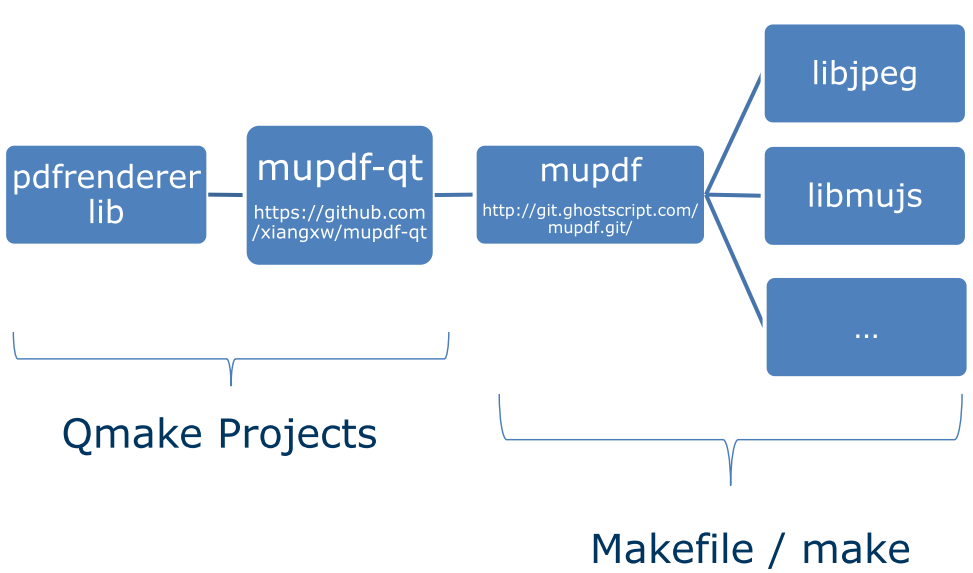
\includegraphics[angle=0,width=14cm]{PdfRenderer/pdfrenderer_aufbau.png}
\caption{Struktur und Aufbau des PDF-Renderer}
%\label{Ladeschluss}
\end{figure}


 


% !TeX encoding = UTF-8
\chapter{Gestensteuerung}
\thispagestyle{fancy}

Die Gestensteuerung hat die Aufgabe Handbewegungen über eine Smartphone-Kamera zu erkennen. Dabei werden zwei Richtungen erkannt und Signale zum vor- und zurückblättert von PDF-Seiten gesendet. Auf Grund der Vorlesung und Recherchen im Internet war schnell klar, dass \href{http://opencv.org/}{OpenCV} eine zweckmäßige Bibliothek darstellt. Als Qt Basis wurde die Version 5.7 und OpenCV in der Version 3.1 verwendet. Der Code für die Gestenerkennung befindet sich unter folgendem \href{https://github.com/BeckmaR/EmbeddedMultimediaSS2016/tree/master/src/handcontrol}{Link}. Hierbei wurde ein C++ Klasse "`handcontrol"' erstellt, welche in die App eingebunden ist.

\section{Auslesen von Videoframes aus einer Kamera}
Im Laufe des Projektes stellte sich heraus, dass die Einbindung der Kamera, auf den verschiedenen Plattformen Windows und Android, die größte Herausforderung darstellt. Die Windows Unterstützung wurde hauptsächlich ausgewählt, um den Algorithmus nicht umständlich auf einem Android Gerät jedes mal testen zu müssen. Die Implementierung auf der Windows-Plattform war relativ einfach, da OpenCV schon eine Funktion \href{http://docs.opencv.org/3.1.0/d8/dfe/classcv_1_1VideoCapture.html}{VideoCapture} bietet, welche einzelne Videoframes aus eine Kamera auslesen kann und diese in einer Matrix abspeichert. Diese Methode funktionierte leider nicht auf einen Android-Gerät. Hinweise: nachfolgende Funktionsweisen beziehen sich auf den Entwicklungsstand vom 20.7.2016, ggf. sind schon Bugs behoben oder neue Möglichkeiten zur Kameraauswertung hinzugekommen. Vom Autor wurden unterschiedlichste Varianten zum Auslesen der Kamera über mehrere Stunden untersucht. Von Qt werden hauptsächlich \href{http://doc.qt.io/qt-5/videooverview.html}{zwei Möglichkeiten} für das Auslesen eines VideoFrames angeboten. \href{http://doc.qt.io/qt-5/qabstractvideosurface.html}{QAbstractVideoSurface} definiert eine abstrakte C++ Klasse welche die Funktion present() beinhaltet, welcher die einzelnen Videoframes nacheinander übergeben werden. Ähnlich verhält es sich mit \href{http://doc.qt.io/qt-5/qvideoprobe.html}{QVideoProbe} wobei man hier die Verbindung über ein Connect() mit Signal und Slot hergestellt werden muss. Eine weitere Möglichkeit besteht seit Qt 5.5 darin, ein Video Filter\footnote{\label{video_filter}https://blog.qt.io/blog/2015/03/20/introducing-video-filters-in-qt-multimedia/} in QML zu verwenden und mit Hilfe der Klasse \href{http://doc.qt.io/qt-5/qabstractvideofilter.html}{QAbstractVideoFilter} die einzelnen Videoframes in C++ zu analysieren und ggf. wieder nach QML zu transformieren. Die C++ QCamera funktioniert nicht auf Android-Geräten (\href{https://bugreports.qt.io/browse/QTBUG-41194}{1},\href{http://stackoverflow.com/questions/28041741/qt-qml-camera-to-c-qimage-on-android}{2}), sodass auf das in QML integrierte Camera Objekt zurückgegriffen wird. Bei der QAbstractVideoFiler Variante konnten die Videodaten in Android nicht in den CPU-Adressraum gemappt werden. Mit QVideoProbe war dies möglich. Hierbei wird aus QML das QCamera Objekt in C++ adressierbar gemacht und mit dem QVideoProbe verbunden. Seit Qt 5.6 existiert ein VideoOutput Objekt in QML welches das Auslesen und Anzeigen von VideoFrames steuert, sodass das hier angegebene \href{http://stackoverflow.com/questions/28041741/qt-qml-camera-to-c-qimage-on-android/33238150\#33238150}{Beispiel} noch um ein VideoOutput Objekt ergänzt werden muss. Um keine größeren Unterschiede zwischen dem Algorithmus für die Windows- und der Androidversion zu haben, ist es wünschenswert beide Cameras über Qt auslesen zu lassen. Leider funktioniert der oben für Android vorgestellte Ansatz für Windows nicht. Hier ist ein Workaround mit einer C++ QCamera und dem QAbstractVideoSurface nötig, um ein QVideoFrame zu erhalten. Die neue Variante mit dem "`Video Filter"' wurde auch untersucht, hat aber nur auf ein paar Androidgeräten funktioniert \href{https://bugreports.qt.io/browse/QTBUG-47934/}{QTBUG-47934}. Anscheinend gibt es dort noch Fehler in dem Qt-Framework. Unter folgendem \href{https://wiki.qt.io/Qt_5.7_Multimedia_Backends}{Link} gibt es eine Auflistung welche Funktionen in dem Qt-Multimedia-Framework-5.7 auf den verschiedenen Plattformen aktuell funktionieren.

\subsection{Verbesserungen}
Die mit Qt 5.5 eingeführten Video Filter scheinen ein gute Weg zu sein, um VideoFrames in Qt analysieren zu können. Leider ist aktuell die Implementierung nicht auf allen Androidgeräten funktional, sodass auf ein Workaround mit QVideoProbe zurückgegriffen werden musste. Diese Variante ist aber leider nicht optimal, da sie Verzögerungen zwischen dem Aufnehmen und dem Aufruf der Funktion present() enthält\footnote{https://blog.qt.io/blog/2015/03/20/introducing-video-filters-in-qt-multimedia/\#comment-1195419}. Eine weitere Möglichkeit besteht, QML \href{http://doc.qt.io/qt-5/qml-qtquick-shadereffect.html}{ShaderEffect} mit OpenGL zu verwenden. Da die Android Kamera seine Videoframes auf der Grafikkarte in OpenGL Texture vorhält \footnote{https://blog.qt.io/blog/2015/03/20/introducing-video-filters-in-qt-multimedia/\#comment-1195414}, wäre es sinnvoll diese auch dort weiter zu verarbeiten. Das kann seit neuem mit Video Shader Objekten direkt in QML programmiert werden. Außerdem war es dem Autor über QML nicht möglich exakte Auflösungen und Frameraten einzustellen. Anscheinend ignoriert Qt gewisse Parameter auf verschiedenen Platformen oder es stehen nicht alle Einstellung zur Verfügung. Jedenfalls sind diese nicht richtig dokumentiert. Ein Problem ist außerdem, dass es vorkommen kann das Frameraten von 30 fps auf 16 fps einbrechen oder kein reproduzierbares Verhalten zeigen. Dieser Punkt konnte innerhalb der Arbeit leider nicht geklärt werden. Eine andere Möglichkeit, welche nicht weiter verfolgt wurde, wäre über Qt mit den \href{http://doc.qt.io/qt-5/qtandroidextras-module.html}{Qt Android Extras} die Androidkamera über Java Code in die Qt Anwendung einzubetten, ggf. auch über das vorhandene OpenCV Java Binding. 

\section{Handerkennungsalgorithmus}
Aus Qt liegen die QVideoFrames als RGB (Windows) und als YUV420 (Android) vor. Diese werden als erstes in Grauwertbilder umgewandelt. Bei dem Android QVideoFrame muss keine pixelweise Konvertierung durchgeführt werden, sondern es wird nur der Luminanz Y Teil des Bildes genommen. Anschließend wird das Differenzbild zwischen dem aktuellen und vorherigen Grauwertbild berechnet. Hierbei achtet OpenCV selbständig darauf, dass eine Sättigung im Zahlenbereich durchgeführt wird.

\begin{figure}[ht!]
\centering
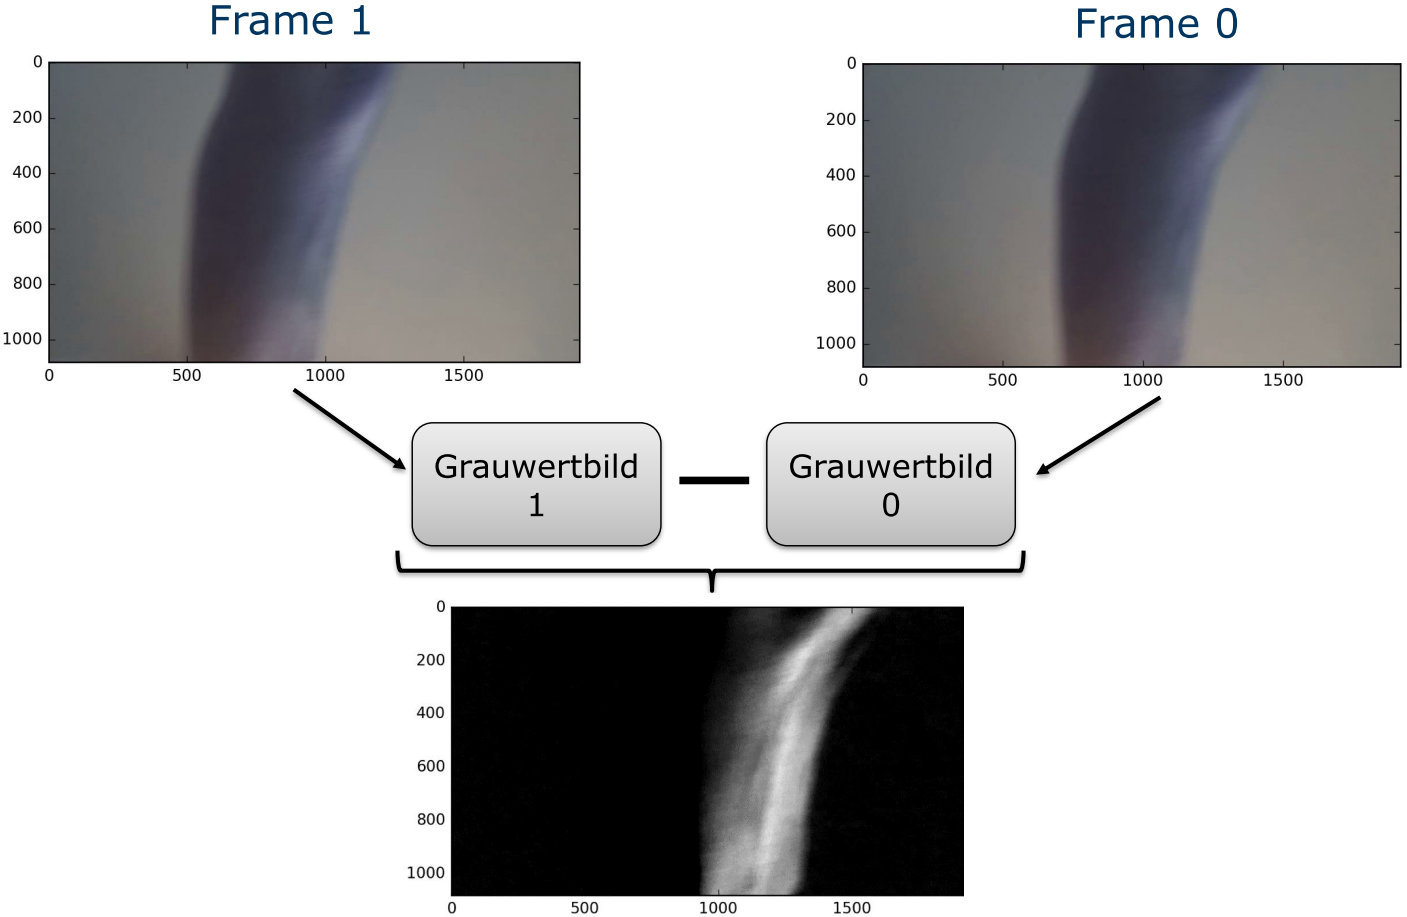
\includegraphics[angle=0,width=14cm]{handcontrol/Bilder/diff_frame1-frame0.png}
\caption{Differenzberechnung zwischen aktuellem und vorherigen Grauwertbild}
\end{figure}

Im nachfolgenden Schritt wir mit Hilfe der reduce() Funktion von OpenCV ein Mittelwert über alle Spalten gebildet. Man erhält einen Zeilenvektor wobei jeder Eintrag den Mittelwert eine Spalte repräsentiert. Hierbei kann man schnell erkennen wo sich in der Horizontalen die größten Änderungen ergeben. Das nennt der Autor Histogramm, da es die Häufigkeitsverteilung darstellt.

\begin{figure}[ht!]
\centering
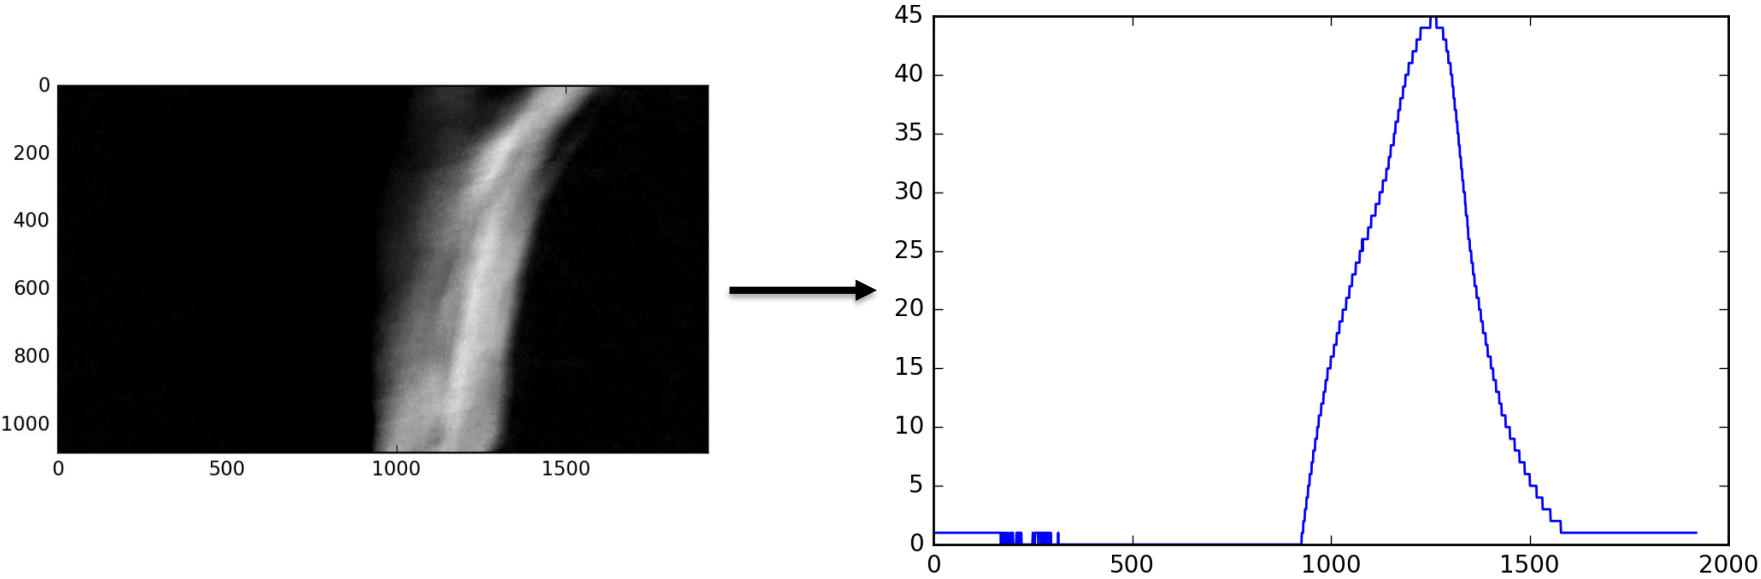
\includegraphics[angle=0,width=14cm]{handcontrol/Bilder/diff_frame_to_hist.png}
\caption{Berechnung des Histogramms über die Spalten eines Differenzbildes}
\end{figure}

Untersucht man die Verschiebung des Histogramms über die Horizontalen, kann man Handbewegungen erkennen. Hierbei wird als erstes der Schwerpunkt des Histogramms gebildet. Das geschieht mit Hilfe einer kumulierten Summe über alle Histogrammwerte. Würde man nur den maximalen Wert des Histogramms betrachten, kann bei verrauschten Bildern eine zu große Abweichung auftreten. Vor dem Berechnen des Schwerpunktes wird noch ein konstanter Faktor subtrahiert, um den ggf. existierenden Rauschteppich zu entfernen. Zur weiteren Fehlerreduktion wurden im folgenden nur diese Schwerpunkte ausgewählt, welche auch mindestens einen gewissen maximalen Histogrammwert aufweisen. Der Wert kann im Sourcecode nachgelesen werden. Um auszuwerten, ob eine PDF vor- oder zurückgeblättert werden soll, untersucht der Algorithmus zeitlich aufeinanderfolgende Schwerpunkte von Histogrammen der Differenzbilder. Er sendet ein Signal, wenn ohne Unterbrechung der Schwerpunkt eine gewisse Zeit in eine der beiden Richtungen gewandert ist. Um den GUI-Thread nicht zu überlasten und um eine flüssige Bedienung der GUI sicher zu stellen, wurde der Algorithmus in ein QThread verschoben. Der so beschriebene Algorithmus benötigt mit 30 Frames pro Sekunde auf Windows ~7ms und auf Android ~10 ms. Somit ist die Echtzeitfähigkeit gegeben. Als Alternative zum dem Differenzbild wurde auch der in OpenCV implementierte Background Substraction Algorithmus (\href{http://docs.opencv.org/3.0-rc1/d7/d7b/classcv_1_1BackgroundSubtractorMOG2.html}{BackgroundSubtractorMOG2}) untersucht. Dieser schätzt den Hintergrund über gaußsche Mischungsverhältnisse mit Mittelwert und Kovarianzmatrix. Leider benötigt der Algorithmus viel Berechnungszeit (~14 Windows und ~30 ms Android) und kratzt somit bei Android Geräten an der Echtzeitfähigkeit. Außerdem würde eine solche Implementierung zu viel Energie des Akkus verbrauchen und wurde deshalb verworfen.

\begin{figure}[ht!]
\centering
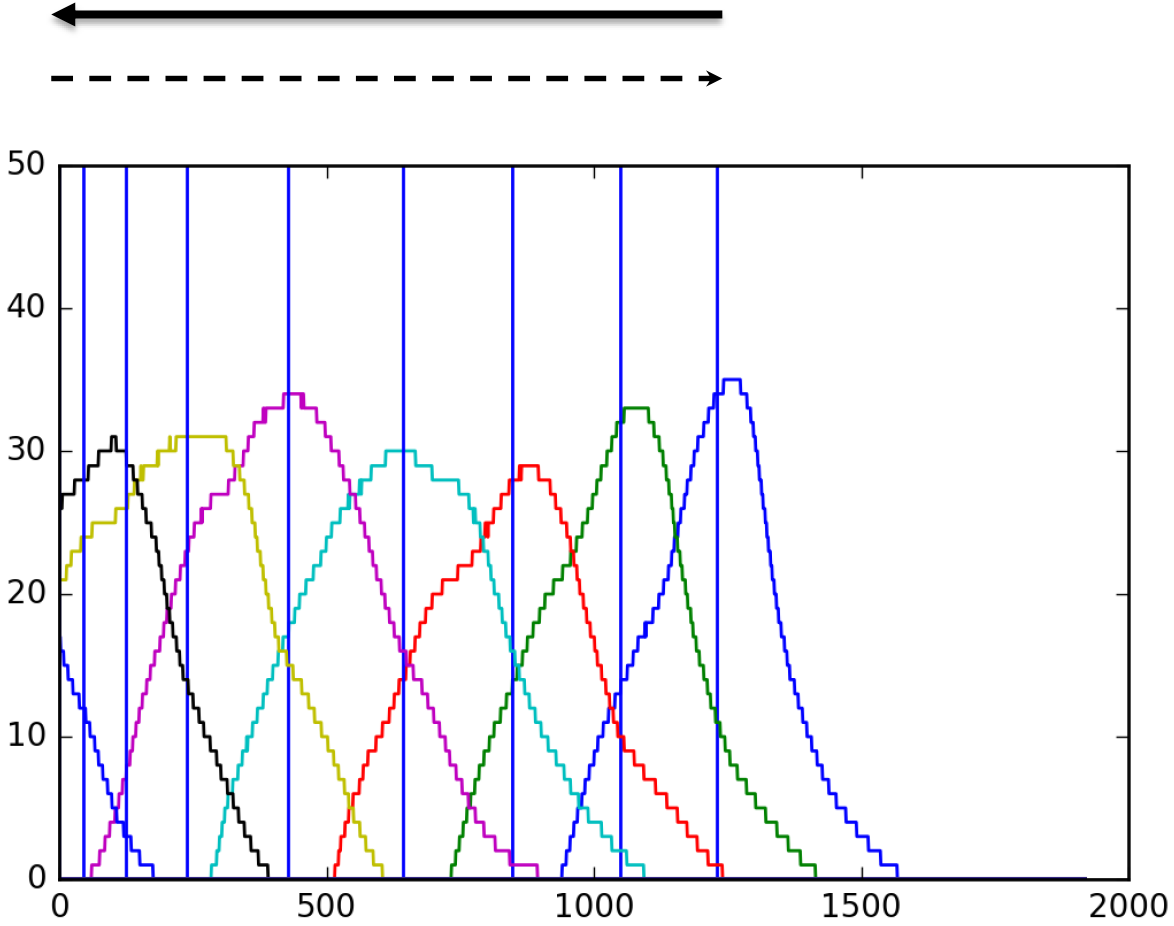
\includegraphics[angle=0,width=14cm]{handcontrol/Bilder/histogramm_schwerpunkt.png}
\caption{Histogramme der Differenzbilder mit Schwerpunkt}
\end{figure}

\section{Entwicklung des Algorithmus}
Der Algorithmus wurde als erstes in MATLAB mit aufgenommenen Videos entwickelt. Nachher wurde auf Python mit OpenCV Binding umgestellt, um einen besseren Vergleich mit der C++ Version zu gewährleisten. Als IDE für Python wurde \href{https://github.com/spyder-ide/spyder}{Spyder} mit dem \href{https://www.continuum.io/downloads}{Anaconda Framework} verwendet. Um den Algorithmus separat von der App zu entwickeln wurde ein "`test\_handcontrol.pro"' Projekt erstellt, welches als eine Art Modultest fungiert. Zu finden in dem schon am Anfang des Kapitels genannten Verzeichnis in Github.

\section{Verbesserungen}
Die Verbesserungen zum Auslesen der Kamera wurden schon in einem separaten Abschnitt behandelt. Für den Algorithmus könnte man statt Grauwertbilder auch Bilder aus dem HSV Raum verwenden. Dort könnte man ggf. Helligkeitsveränderung besser abfangen. Außerdem kann es manchmal vorkommen, dass mehrfach Erkennung erfolgen, diese könnten durch einen Timer abgefangen werden. Eine Verschiebung der Berechnung zur Grafikkarte mittels OpenGL oder OpenCL, wie vorher schon erwähnt, könnte die CPU entlasten und ganz andere Möglichkeiten der Analyse des Frames bieten. Bei der Differenzbildung der Frames entstehen positive und negative Abweichungen, diese könnten in einem verbesserten Algo. separat berücksichtigt werden.


\chapter[server]{Der Server}
\section{Zweck und Aufgaben des Servers}
Der Server stellt die Komponente dar, welche die diversen Endgeräte per Netzwerk miteinander verbindet und verwaltet. Hierbei ist im Folgenden von "`Clients"' die Rede, wenn es um die Menge aller verbundenen Geräte geht. Der "`Master"' stellt den Sprecher dar, welcher eine Präsentation hochladen darf sowie die aktuell angezeigte Seite ändern. Alle anderen Geräte haben lediglich eine Zuhörer-Funktion.

Er authorisiert den Sprecher, der sich mit dem gültigen Master-Passwort anmelden möchte, und erlaubt nach erfolgter Anmeldung das Hochladen einer Präsentation und Steuern der anzuzeigenden Seitenzahl. Die Präsentation wird gleichzeitig auch auf dem Desktop angezeigt, so dass der Server per Monitorkabel an ein Anzeigegerät - z.B. einen Beamer - angeschlossen werden kann um die Präsentation auszugeben. In diesem Projekt lief die Server-Software auf einem Raspberry Pi.

Per Netzwerk wird die Präsentation sowie die anzuzeigende Seitenzahl auf Anforderung an die Clients verteilt, so dass jeder Client die Präsentation synchron mitverfolgen kann.

Nachdem sich ein Master von dem Server getrennt hat, ist das Verbinden eines neuen Mastergerätes ohne Probleme möglich. Dies erlaubt es, nacheinander mehrere Sprecher eine Präsentation halten zu lassen, ohne dass die Server-Software neugestartet wird. Das gleichzeitige Verbinden mehrerer Sprecher ist hingegen nicht möglich, um Verwirrungen und komplizierte Rechteverwaltungen zu vermeiden.

\section{Das Konzept}
Die Implementierung der Netzwerkverbindung erfolgte auf Basis von Websockets. Dies ist ein auf TCP basierendes Protokoll, bei dem eine bidirektionale Datenverbindung möglich ist. Die Verbindung wird außerdem aufrecht erhalten - dies ermöglicht es, serverseitig die Verbindung zum Master separat abzuspeichern. So wird nicht bei jeder Aktion eine Authentifizierung benötigt. Außerdem könnte ein Server, der nicht-persistente Verbindungen verwendet, nicht die aktuelle Seitenzahl an alle Clients broadcasten - er kennt seine Clients gar nicht, und jede Aktion wird von den Clients eingeleitet. Diese müssten beispielsweise alle $x$ Sekunden den Server pollen, um die aktuelle Seitenzahl zu erfragen.

Diese Technik stellt also kein \textit{Stateless Design} dar, sondern einen sehr simplen Zustandsautomaten.

\subsection{Kommunikationsprotokoll}
Mit Hilfe der Qt-Implementierung von Websockets, den \verb+QWebSocket+s, lassen sich Text- und Binärnachrichten versenden. Auf dieser Basis wurde ein sehr einfaches textbasiertes Protokoll für die Kommunikation zwischen Server und Client entwickelt. Die folgenden Befehle können vom Client an den Server gesendet werden, dieser antwortet dann an diesen oder alle Clients.

Alle Kommandos folgen einem einheitlichen Format: Zwei Zeichen, gefolgt von einem Doppelpunkt und weiteren Zeichen beliebiger Länge (einschließlich Länge 0, also keine weiteren Zeichen). Die beiden Zeichen vor dem Doppelpunkt definieren, was getan werden soll, und die weiteren Zeichen stellen die "`Payload"' dar, wie zum Beispiel weitere Argumente oder das Passwort bei dem Versuch sich als Master anzumelden.
\begin{itemize}
	\item \verb+RM+ - \textbf{R}egister as \textbf{M}aster.
		\begin{description}
			\item[Payload] Das korrekte Master-Passwort.
			\item[Fehlermeldungen] \verb+BADPW+ bei falschem Passwort, \verb+MASTERISSET+ wenn es bereits einen Master gibt - per WebSocket an den Client gesendet
			\item [Erfolgsbestätigung] \verb+ACK+
			\item [Beispiele] Korrekt: \verb+RM:mpw12345+, nicht korrekt: \verb+RM:123+
		\end{description}
	\item \verb+SP+ - \textbf{S}et \textbf{P}age.
		\begin{description}
			\item[Payload] Eine Seitenzahl, die sich in einen integer umwandeln lässt.
			\item[Fehlermeldungen] \verb+BADPAGENUM+ bei ungültigen Seitenzahlen, die nicht zu einem integer gewandelt werden konnten, \verb+NOTALLOWED+ wenn der Sender nicht als Master registriert ist.
			\item [Erfolgsbestätigung] Broadcast der Seitenzahl an alle (Weiterleitung)
			\item [Beispiele] Korrekt: \verb+SP:3+, nicht korrekt: \verb+SP:x+
		\end{description}
	\item \verb+GP+ - \textbf{G}et \textbf{P}age.
		\begin{description}
			\item[Payload] Wird ignoriert, nichts notwendig. 
			\item[Fehlermeldungen] Wenn noch kein pdf verfügbar ist, wird die Default-Seitenzahl '-1' gesendet.
			\item [Erfolgsbestätigung] Antwort mit \verb+PN:X+, wobei $X$ die Seitenzahl bezeichnet.
			\item [Beispiele] Korrekt: \verb+GP:+, oder auch korrekt: \verb+GP:x+ - Payload wird ignoriert
		\end{description}
	\item \verb+DL+ - \textbf{D}own\textbf{l}oad.
		\begin{description}
			\item[Payload] Wird ignoriert.
			\item[Fehlermeldungen] \verb+NOFILE+, wenn keine Präsentation hochgeladen wurde.
			\item [Erfolgsbestätigung] Der Inhalt der Datei wird per BinaryMessage an den Client geschickt.
			\item [Beispiele] Korrekt: \verb+DL:+,
		\end{description}
	\item \verb+UL+ - \textbf{U}p \textbf{L}oad. Kann verwendet werden, um zu erfragen, ob ein Upload erlaubt ist.
		\begin{description}
			\item[Payload] Wird ignoriert.
			\item[Fehlermeldungen] \verb+NOTALLOWED+ wenn der Sender nicht als Master registriert ist.
			\item [Erfolgsbestätigung] \verb+ACK+
			\item [Beispiele] Korrekt: \verb+DL:+
		\end{description}
	\item Die Präsentation hochladen. Dies ist kein Textkommando, sondern erfolgt direkt per BinaryMessage. Diese wird nur akzeptiert, wenn der Sender der aktuelle Master ist. In diesem Fall wird das enthaltene \verb+QByteArray+ direkt an den pdfrenderer weitergeleitet, welcher dieses dann in eine Datei schreibt und anzeigt.
\end{itemize}
Andere Kommandos werden generell mit \verb+BADCMD+ beantwortet.

\section{Mögliche Verbesserungen}
Der Server erledigt seine Aufgabe recht gut. Die Schnittstelle ist möglichst simpel gehalten und weist eine geringe Fehleranfälligkeit auf. Diverse Funktionen für die Sicherheit oder Annehmlichkeiten wären aber noch vorstellbar.

\begin{itemize}
	\item Verschlüsselte Verbindung. Das Master-Passwort wird, wie alles andere auch, per Klartext übertragen. Während der Präsentation ist ein weiterer Master nicht erlaubt, danach könnte ein potentieller Angreifer sich aber anmelden.
	\item Broadcast des Servers. Der Server könnte in regelmäßigen Abständen per UDP-Broadcast auf sich aufmerksam machen. Dadurch könnten Clients sich automatisch verbinden, und das unelegante Eintippen der ip-Adresse im Client würde entfallen.
	\item Zuteilung einer ID zu einem Master. Mit dieser ID könnte ein Master sich nach einem Verbindungsabbruch neu verbinden und an der vorherigen Stelle weitermachen.
\end{itemize}




\chapter[Zusammenfassung und Ausblick]{Zusammenfassung und Ausblick\footnote{Jens Helge Micke}}
\thispagestyle{fancy}
\label{Ausblick}

%\addcontentsline{toc}{chapter}{Danksagung}
%\include{Danksagung/Danksagung}

\addcontentsline{toc}{chapter}{Literaturverzeichnis}
\bibliography{Literaturverzeichnis/biblio}
\bibliographystyle{Literaturverzeichnis/unsrtdin_pi}

\end{document}
